\chapter{Method}

In this chapter we present our methodology for fulfilling the aim of developing accurate models for predicting age and sex, and how they can be analysed in order to gain insight into what functional networks are related to age and sex differences in the human brain. The chapter can be summarised as follows: First, we present the preprocessing of the fMRI data into graphs suitable for neural networks. Secondly, models for graph and node prediction are presented. Finally, methods for analysing the models are presented.

\section{From fMRI scans to graphs}\label{sec:fmri_to_graphs}
The data that makes up the foundation of this master thesis is from the UK Biobank \cite{ukbiobank}. The UK Biobank is an extensive data bank that contains genetic and biomedical information for over 500 000 individuals in the UK. Examples of types of data that are included in the biobank are subject sex, age, cognitive abilities, disease history, but also more specific information such as MRI and fMRI brain scans.

\todo{Byt färg på orange/blå i figuren om vi verkligen vill använda den här som atlas. Just nu okej, eftersom den bara är schematisk, men annars är den inkorrekt. }
\begin{figure}[H]
    \centering
    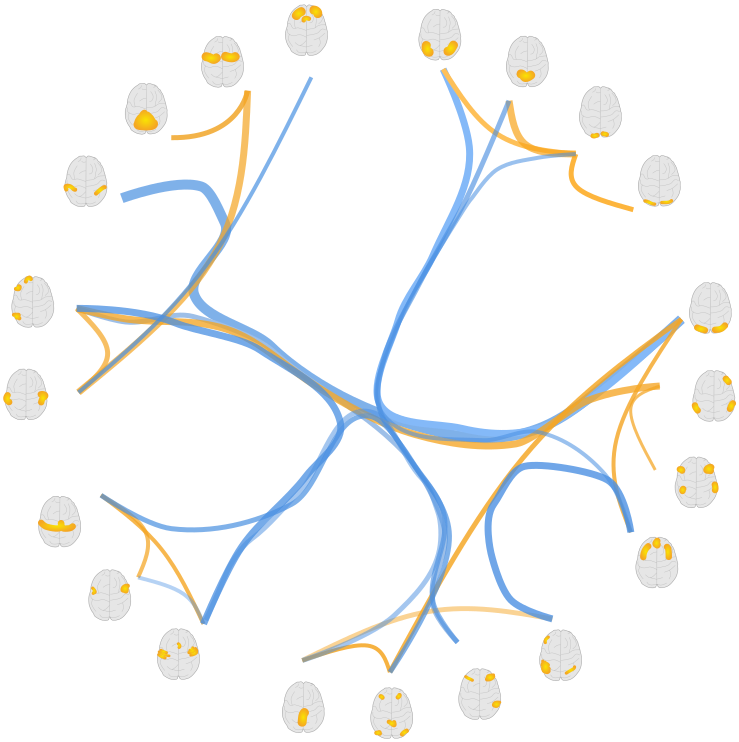
\includegraphics[width=0.6\textwidth]{chapters/images_methods/fmri_network_redone.png}
    \caption{A schematic visualisation of a network of functional brain networks. Blue and orange edges represent positive and negative correlation between brain networks, respectively.  The individual functional brain networks are represented as human brains with fictive fMRI activations (orange), along the circumference of the circle. Image created with inspiration from example at UK Biobank brain imaging showcase  \cite{ukbiobank_brain_imaging}.}
    \label{fig:fmri_network}
\end{figure}

In the UK Biobank, fMRI brain scans, which are the focus of this project, are available for roughly 35 000 subjects varying between 45 and 80 years of age. Functional MRI (fMRI) is a technique for measuring the activation of the human brain \cite{sporns}. In a measurement, the activation of various parts of the subject brain is measured as time series. The correlation between these time series can then be calculated, and highly correlated regions can be formed into networks. The regions that make up these network does not necessarily have to be physically close together. The obtained fMRI brain networks are often associated with certain functionalities of the brain. One example of such a functional brain network is the Default Mode Network (DMN), which handles memory processing and mind wandering \cite{alves_dmn}. 

The fMRI data available from the UK Biobank for this project has also been further preprocessed. fMRI networks that are related to the same functional brain network have been clustered together to form a 21 node \textit{network of networks}, which is represent as a graph. Each node in the brain graphs thus corresponds to one functional network in the human brain (such as the DMN etc.). The weight of the edges between each of the nodes is calculated as the average correlation between the networks that make up the two nodes. Thus, weights can both be positive and negative, depending on the correlation. A visualization of such a brain graph is given in figure \ref{fig:fmri_network}, in which the various nodes and the functional brain networks they represent form the outer circle, with the coloured lines connecting the nodes being the edges in the graph. The lines are coloured according to edge weight, with blue and orange lines having positive and negative weight respectively.

\subsection{How to handle negative values - split}

A brain graph with both positive and negative weights may however be problematic. Specifically, when normalizing the adjacency matrices according to equation \eqref{eq:renormalization_trick}, the risk of dividing by zero becomes imminent. There are several ways to handle this problem. One alternative is to only study all positive or all negative connections, and another might be to take the absolute value of all connections. We however decided to split the negative and positive connections into two separate graphs and thus form a multiplex graph. From a practical point of view this was implemented by creating a block diagonal adjacency matrix $A_{split}$ with all positive connections in the upper block and all negative connections in the lower block, see figure \ref{fig:block_diagonal_adjacency_matrix}. The connections in the positive block that were negative in the original adjacency matrix $A$ were replaced with zeros, and vice versa in the negative block.

\begin{figure}[H]
    \centering
    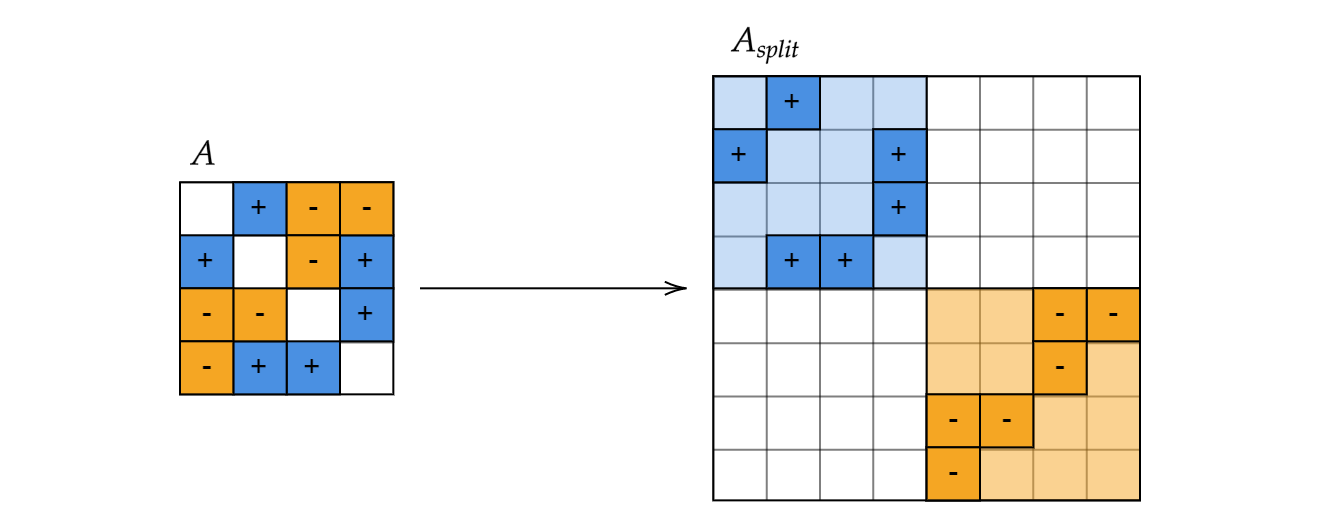
\includegraphics[width=0.9\textwidth]{chapters/images_methods/split.png}
    \caption{An example of how negative values in an adjacency matrix $A$ are handled. The negative values (orange) are extracted into the lower diagonal block, and replaced with zeros in the upper, positive block (blue).}
    \label{fig:block_diagonal_adjacency_matrix}
\end{figure}

\section{Graph classification -- subject-wise}

Having described the preprocessing of the brain graphs, we now turn to the models used to perform graph prediction for individual subjects. Two models will be presented, a baseline regression model and a GCN-based model, for the tasks of predicting subject age and sex.

\subsection{Baseline model}
To be able to validate how well the different GCN-models performs a baseline model must be introduced for comparison. In this study the baseline model consisted of a regression model where the connections between all of the nodes were regarded as separate input features. The adjacency matrix for an individual subject could then be viewed as a high dimensional data point and the model thus aimed to fit a hyper plane to either separate the classes or predict a continues variable. For a schematic view of the model see figure \ref{fig:Graph_class_baseline}. Note specifically that the output layer has either two softmax-activated neurons in the case of sex classification or one neuron without activation in the case of age regression. 

As described in \ref{sec:general_graph_theory} graphs are completely node invariant, and several different ways of listing the connections results in the same graph. This might generally impose a problem since the regression model depend on its input being ordered. The reason a regression model is possible as a baseline in this case, is because the brain graphs from the UK Biobank follows a consistent node ordering, and each input feature of the model is thus always the same connection. Another reason this baseline model is possible is because the brain graphs are relative small (21 nodes) compared to many other graphs (citetion networks for example). For larger graphs, models with one learnable parameter per connection would result in huge models. In that case models that do not scale with the number of connections must be used, such as GCN-based models. 

% \begin{center}
%     \resizebox {0.9\linewidth} {!} {
%         

\tikzset{every picture/.style={line width=0.75pt}} %set default line width to 0.75pt        

\begin{tikzpicture}[x=0.75pt,y=0.75pt,yscale=-1,xscale=1]
%uncomment if require: \path (0,256); %set diagram left start at 0, and has height of 256

%Straight Lines [id:da08012385894546048] 
\draw [color={rgb, 255:red, 0; green, 0; blue, 0 }  ,draw opacity=1 ]   (45,45) -- (185,130) ;
%Straight Lines [id:da8398961471148605] 
\draw [color={rgb, 255:red, 0; green, 0; blue, 0 }  ,draw opacity=1 ]   (45,85) -- (185,130) ;
%Straight Lines [id:da8832621988467466] 
\draw [color={rgb, 255:red, 0; green, 0; blue, 0 }  ,draw opacity=1 ]   (45,125) -- (185,130) ;
%Straight Lines [id:da8658449844223002] 
\draw [color={rgb, 255:red, 0; green, 0; blue, 0 }  ,draw opacity=1 ]   (45,215) -- (185,130) ;
%Straight Lines [id:da9842325204560114] 
\draw    (220,130) -- (270,130) ;
%Straight Lines [id:da9699253287015002] 
\draw    (280,110) -- (270,130) ;
%Straight Lines [id:da3136144075299854] 
\draw    (270,130) -- (280,150) ;
%Straight Lines [id:da4214591700017929] 
\draw    (280,110) -- (318,110) ;
\draw [shift={(320,110)}, rotate = 180] [fill={rgb, 255:red, 0; green, 0; blue, 0 }  ][line width=0.08]  [draw opacity=0] (12,-3) -- (0,0) -- (12,3) -- cycle    ;
%Straight Lines [id:da7746738186045765] 
\draw    (280,150) -- (318,150) ;
\draw [shift={(320,150)}, rotate = 180] [fill={rgb, 255:red, 0; green, 0; blue, 0 }  ][line width=0.08]  [draw opacity=0] (12,-3) -- (0,0) -- (12,3) -- cycle    ;
%Shape: Axis 2D [id:dp11393948673287424] 
\draw  (430,122.25) -- (460,122.25)(433,97.47) -- (433,125) (453,117.25) -- (460,122.25) -- (453,127.25) (428,104.47) -- (433,97.47) -- (438,104.47)  ;
%Straight Lines [id:da09576460905063744] 
\draw [color={rgb, 255:red, 74; green, 144; blue, 226 }  ,draw opacity=1 ]   (430,125) -- (451.67,103.33) -- (460,95) ;
%Shape: Axis 2D [id:dp12724162882260592] 
\draw  (430,157.07) -- (460,157.07)(433,135) -- (433,159.53) (453,152.07) -- (460,157.07) -- (453,162.07) (428,142) -- (433,135) -- (438,142)  ;
%Straight Lines [id:da9285983842245029] 
\draw [color={rgb, 255:red, 208; green, 2; blue, 27 }  ,draw opacity=1 ]   (440,137) -- (440,157) ;
%Straight Lines [id:da4541122584680737] 
\draw [color={rgb, 255:red, 74; green, 144; blue, 226 }  ,draw opacity=1 ]   (450,147) -- (450,157) ;

%Shape: Circle [id:dp5473399963870353] 
\draw  [fill={rgb, 255:red, 255; green, 255; blue, 255 }  ,fill opacity=1 ] (30,45) .. controls (30,36.72) and (36.72,30) .. (45,30) .. controls (53.28,30) and (60,36.72) .. (60,45) .. controls (60,53.28) and (53.28,60) .. (45,60) .. controls (36.72,60) and (30,53.28) .. (30,45) -- cycle ;
%Shape: Circle [id:dp9366596747620268] 
\draw  [fill={rgb, 255:red, 255; green, 255; blue, 255 }  ,fill opacity=1 ] (30,215) .. controls (30,206.72) and (36.72,200) .. (45,200) .. controls (53.28,200) and (60,206.72) .. (60,215) .. controls (60,223.28) and (53.28,230) .. (45,230) .. controls (36.72,230) and (30,223.28) .. (30,215) -- cycle ;
%Shape: Circle [id:dp6370056516541169] 
\draw  [fill={rgb, 255:red, 255; green, 255; blue, 255 }  ,fill opacity=1 ] (30,125) .. controls (30,116.72) and (36.72,110) .. (45,110) .. controls (53.28,110) and (60,116.72) .. (60,125) .. controls (60,133.28) and (53.28,140) .. (45,140) .. controls (36.72,140) and (30,133.28) .. (30,125) -- cycle ;
%Shape: Circle [id:dp6076795307057334] 
\draw  [fill={rgb, 255:red, 255; green, 255; blue, 255 }  ,fill opacity=1 ] (30,85) .. controls (30,76.72) and (36.72,70) .. (45,70) .. controls (53.28,70) and (60,76.72) .. (60,85) .. controls (60,93.28) and (53.28,100) .. (45,100) .. controls (36.72,100) and (30,93.28) .. (30,85) -- cycle ;
%Shape: Circle [id:dp15718416196861162] 
\draw  [fill={rgb, 255:red, 255; green, 255; blue, 255 }  ,fill opacity=1 ] (150,130) .. controls (150,110.67) and (165.67,95) .. (185,95) .. controls (204.33,95) and (220,110.67) .. (220,130) .. controls (220,149.33) and (204.33,165) .. (185,165) .. controls (165.67,165) and (150,149.33) .. (150,130) -- cycle ;

% Text Node
\draw (37,204.4) node [anchor=north west][inner sep=0.75pt]    {$x_{n}$};
% Text Node
\draw (37,114.4) node [anchor=north west][inner sep=0.75pt]    {$x_{3}$};
% Text Node
\draw (37,74.4) node [anchor=north west][inner sep=0.75pt]    {$x_{2}$};
% Text Node
\draw (37,34.4) node [anchor=north west][inner sep=0.75pt]    {$x_{1}$};
% Text Node
\draw (84,57.4) node [anchor=north west][inner sep=0.75pt]  [font=\scriptsize,color={rgb, 255:red, 0; green, 0; blue, 0 }  ,opacity=1 ]  {${\textstyle \theta _{1}}$};
% Text Node
\draw (84,87.4) node [anchor=north west][inner sep=0.75pt]  [font=\scriptsize,color={rgb, 255:red, 0; green, 0; blue, 0 }  ,opacity=1 ]  {${\textstyle \theta _{2}}$};
% Text Node
\draw (84,114.4) node [anchor=north west][inner sep=0.75pt]  [font=\scriptsize,color={rgb, 255:red, 0; green, 0; blue, 0 }  ,opacity=1 ]  {${\textstyle \theta _{3}}$};
% Text Node
\draw (84,157.4) node [anchor=north west][inner sep=0.75pt]  [font=\scriptsize,color={rgb, 255:red, 0; green, 0; blue, 0 }  ,opacity=1 ]  {${\textstyle \theta _{n}}$};
% Text Node
\draw (151,109.4) node [anchor=north west][inner sep=0.75pt]  [font=\footnotesize]  {$\sigma \left(\sum _{i} \theta _{i} x_{i}\right)$};
% Text Node
\draw (380,130) node   [align=left] {\begin{minipage}[lt]{68pt}\setlength\topsep{0pt}
\textbf{Age}
\begin{undefined}
\textit{or}
\end{undefined}
\textbf{Male/Female}
\end{minipage}};
% Text Node
\draw (241,109.4) node [anchor=north west][inner sep=0.75pt]    {$y$};
% Text Node
\draw (34,152.4) node [anchor=north west][inner sep=0.75pt]  [font=\Large]  {$\vdots $};


\end{tikzpicture}

%     }
% \end{center}

\begin{figure}[H]
    \centering
    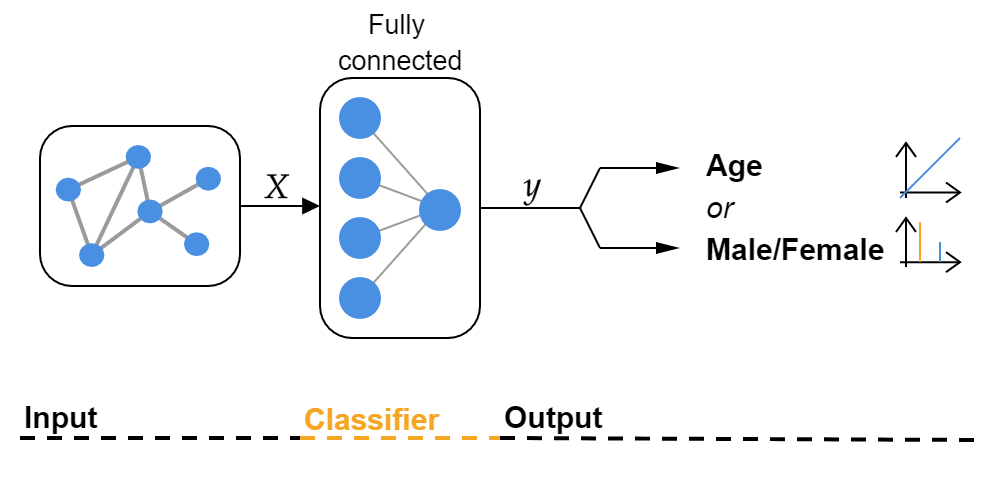
\includegraphics[width=0.9\textwidth]{chapters/images_methods/ffnn_v2.png}
    \caption{The baseline regression model. The adjacency matrix for a brain graph for a single subject forms the input, with a continuous value or class prediction as output in the case of sex or age prediction.}
    \label{fig:Graph_class_baseline}
\end{figure}

\subsection{GCN}

The motivation behind using GCN-based models is that they hopefully will be able to extract information from the topological structure of the graph, rather than simply studying the individual connections as, for instance, in the case of the baseline model. To explore this possibility, a GCN-based model, referred to simply as GCN, was developed. An illustration of the GCN model can be seen in figure \ref{fig:gcn_base}. GCN consisted of three consecutive graph convolutional layers, with propagation rule as defined in equation \eqref{eq:propagation_rule}, followed by a fully connected output layer. The graph convolutional layers had a rectified linear unit (RELU) activation function and ten output features. This will be the case for all graph convolutional layers mentioned in the remainder of the thesis, unless otherwise specified. The input to the fully connected output layer consisted of the activations for all three graph convolutional layers, i.e. the activation for all feature maps in all layers, concatenated together. As described in section \ref{sec:gcn} the activation of layer $i$ contains information about the $i$:th-order neighbourhood of each node. The inclusion of the activations after each layer in the classifier thus aims to utilize information of how each node is embedded in a successively larger neighbourhood, which could be beneficial for the prediction.

As described in section \ref{sec:gcn}, the inputs to a graph convolutional layer consists of an adjacency matrix $A$ and a node feature matrix $X$. In the case of GCN however, a \textit{featureless} approach was used, in which the feature matrix was taken to be the identity matrix, $X=I$, since the fMRI graph is already represented by the adjacency matrix $A$. Other data modalites than fMRI data could be included through the feature matrix $X$, but we opted for the featureless approach due to the focus in this thesis on fMRI data specifically.

% \begin{center}
%     \resizebox {0.9\linewidth} {!} {
%         

\tikzset{every picture/.style={line width=0.75pt}} %set default line width to 0.75pt        

\begin{tikzpicture}[x=0.75pt,y=0.75pt,yscale=-1,xscale=1]
%uncomment if require: \path (0,268); %set diagram left start at 0, and has height of 268

%Rounded Rect [id:dp1454512597044859] 
\draw  [fill={rgb, 255:red, 255; green, 255; blue, 255 }  ,fill opacity=1 ] (150,48) .. controls (150,38.06) and (158.06,30) .. (168,30) -- (222,30) .. controls (231.94,30) and (240,38.06) .. (240,48) -- (240,222) .. controls (240,231.94) and (231.94,240) .. (222,240) -- (168,240) .. controls (158.06,240) and (150,231.94) .. (150,222) -- cycle ;
%Straight Lines [id:da44371133423221676] 
\draw [color={rgb, 255:red, 155; green, 155; blue, 155 }  ,draw opacity=1 ][line width=1.5]    (169.29,109.19) -- (177.86,134.65) ;
%Straight Lines [id:da3398362409006068] 
\draw [color={rgb, 255:red, 155; green, 155; blue, 155 }  ,draw opacity=1 ][line width=1.5]    (169.29,109.19) -- (195,96.46) ;
%Shape: Ellipse [id:dp7222477940626566] 
\draw  [color={rgb, 255:red, 245; green, 166; blue, 35 }  ,draw opacity=1 ][fill={rgb, 255:red, 245; green, 166; blue, 35 }  ,fill opacity=1 ] (165,109.19) .. controls (165,106.85) and (166.92,104.95) .. (169.29,104.95) .. controls (171.65,104.95) and (173.57,106.85) .. (173.57,109.19) .. controls (173.57,111.53) and (171.65,113.43) .. (169.29,113.43) .. controls (166.92,113.43) and (165,111.53) .. (165,109.19) -- cycle ;
%Straight Lines [id:da7434143201874741] 
\draw [color={rgb, 255:red, 155; green, 155; blue, 155 }  ,draw opacity=1 ][line width=1.5]    (199.29,63.23) -- (195,42.02) ;
%Straight Lines [id:da17541088644592207] 
\draw [color={rgb, 255:red, 155; green, 155; blue, 155 }  ,draw opacity=0.4 ][line width=1.5]    (177.86,80.2) -- (195,42.02) ;
%Straight Lines [id:da49554490131335505] 
\draw [color={rgb, 255:red, 155; green, 155; blue, 155 }  ,draw opacity=0.4 ][line width=1.5]    (169.29,54.75) -- (177.86,80.2) ;
%Straight Lines [id:da7823220018723711] 
\draw [color={rgb, 255:red, 155; green, 155; blue, 155 }  ,draw opacity=1 ][line width=1.5]    (199.29,63.23) -- (220.71,50.51) ;
%Straight Lines [id:da4144720186472177] 
\draw [color={rgb, 255:red, 155; green, 155; blue, 155 }  ,draw opacity=0.4 ][fill={rgb, 255:red, 0; green, 0; blue, 0 }  ,fill opacity=0.5 ][line width=1.5]    (169.29,54.75) -- (195,42.02) ;
%Straight Lines [id:da4512038117618906] 
\draw [color={rgb, 255:red, 155; green, 155; blue, 155 }  ,draw opacity=1 ][line width=1.5]    (199.29,63.23) -- (177.86,80.2) ;
%Straight Lines [id:da6717586155874848] 
\draw [color={rgb, 255:red, 155; green, 155; blue, 155 }  ,draw opacity=1 ][line width=1.5]    (199.29,63.23) -- (216.43,75.96) ;
%Shape: Ellipse [id:dp8214542913209517] 
\draw  [color={rgb, 255:red, 167; green, 207; blue, 255 }  ,draw opacity=1 ][fill={rgb, 255:red, 167; green, 207; blue, 255 }  ,fill opacity=1 ] (165,54.75) .. controls (165,52.4) and (166.92,50.51) .. (169.29,50.51) .. controls (171.65,50.51) and (173.57,52.4) .. (173.57,54.75) .. controls (173.57,57.09) and (171.65,58.99) .. (169.29,58.99) .. controls (166.92,58.99) and (165,57.09) .. (165,54.75) -- cycle ;
%Shape: Ellipse [id:dp47038889017471486] 
\draw  [color={rgb, 255:red, 74; green, 144; blue, 226 }  ,draw opacity=1 ][fill={rgb, 255:red, 74; green, 144; blue, 226 }  ,fill opacity=1 ] (173.57,80.2) .. controls (173.57,77.86) and (175.49,75.96) .. (177.86,75.96) .. controls (180.22,75.96) and (182.14,77.86) .. (182.14,80.2) .. controls (182.14,82.55) and (180.22,84.44) .. (177.86,84.44) .. controls (175.49,84.44) and (173.57,82.55) .. (173.57,80.2) -- cycle ;
%Shape: Ellipse [id:dp10306056601214997] 
\draw  [color={rgb, 255:red, 245; green, 166; blue, 35 }  ,draw opacity=1 ][fill={rgb, 255:red, 245; green, 166; blue, 35 }  ,fill opacity=1 ] (195,63.23) .. controls (195,60.89) and (196.92,58.99) .. (199.29,58.99) .. controls (201.65,58.99) and (203.57,60.89) .. (203.57,63.23) .. controls (203.57,65.58) and (201.65,67.47) .. (199.29,67.47) .. controls (196.92,67.47) and (195,65.58) .. (195,63.23) -- cycle ;
%Shape: Ellipse [id:dp3356200716848863] 
\draw  [color={rgb, 255:red, 74; green, 144; blue, 226 }  ,draw opacity=1 ][fill={rgb, 255:red, 74; green, 144; blue, 226 }  ,fill opacity=1 ] (212.14,75.96) .. controls (212.14,73.62) and (214.06,71.72) .. (216.43,71.72) .. controls (218.8,71.72) and (220.71,73.62) .. (220.71,75.96) .. controls (220.71,78.3) and (218.8,80.2) .. (216.43,80.2) .. controls (214.06,80.2) and (212.14,78.3) .. (212.14,75.96) -- cycle ;
%Shape: Ellipse [id:dp9107615531803757] 
\draw  [color={rgb, 255:red, 74; green, 144; blue, 226 }  ,draw opacity=1 ][fill={rgb, 255:red, 74; green, 144; blue, 226 }  ,fill opacity=1 ] (190.71,42.02) .. controls (190.71,39.68) and (192.63,37.78) .. (195,37.78) .. controls (197.37,37.78) and (199.29,39.68) .. (199.29,42.02) .. controls (199.29,44.36) and (197.37,46.26) .. (195,46.26) .. controls (192.63,46.26) and (190.71,44.36) .. (190.71,42.02) -- cycle ;
%Shape: Ellipse [id:dp686194905732459] 
\draw  [color={rgb, 255:red, 74; green, 144; blue, 226 }  ,draw opacity=1 ][fill={rgb, 255:red, 74; green, 144; blue, 226 }  ,fill opacity=1 ] (216.43,50.51) .. controls (216.43,48.16) and (218.35,46.26) .. (220.71,46.26) .. controls (223.08,46.26) and (225,48.16) .. (225,50.51) .. controls (225,52.85) and (223.08,54.75) .. (220.71,54.75) .. controls (218.35,54.75) and (216.43,52.85) .. (216.43,50.51) -- cycle ;
%Straight Lines [id:da4462253100757778] 
\draw [color={rgb, 255:red, 155; green, 155; blue, 155 }  ,draw opacity=1 ][line width=1.5]    (177.86,227.98) -- (195,189.8) ;
%Straight Lines [id:da33046752635028676] 
\draw [color={rgb, 255:red, 155; green, 155; blue, 155 }  ,draw opacity=1 ][line width=1.5]    (169.29,202.53) -- (177.86,227.98) ;
%Straight Lines [id:da45388559372006365] 
\draw [color={rgb, 255:red, 155; green, 155; blue, 155 }  ,draw opacity=1 ][line width=1.5]    (199.29,211.01) -- (177.86,227.98) ;
%Shape: Ellipse [id:dp12334564292514116] 
\draw  [color={rgb, 255:red, 245; green, 166; blue, 35 }  ,draw opacity=1 ][fill={rgb, 255:red, 245; green, 166; blue, 35 }  ,fill opacity=1 ] (173.57,227.98) .. controls (173.57,225.64) and (175.49,223.74) .. (177.86,223.74) .. controls (180.22,223.74) and (182.14,225.64) .. (182.14,227.98) .. controls (182.14,230.32) and (180.22,232.22) .. (177.86,232.22) .. controls (175.49,232.22) and (173.57,230.32) .. (173.57,227.98) -- cycle ;
%Straight Lines [id:da5879944549609841] 
\draw [color={rgb, 255:red, 155; green, 155; blue, 155 }  ,draw opacity=0.4 ][fill={rgb, 255:red, 0; green, 0; blue, 0 }  ,fill opacity=0.5 ][line width=1.5]    (195,96.46) -- (177.86,134.65) ;
%Straight Lines [id:da10478801456064013] 
\draw [color={rgb, 255:red, 155; green, 155; blue, 155 }  ,draw opacity=0.4 ][fill={rgb, 255:red, 0; green, 0; blue, 0 }  ,fill opacity=0.5 ][line width=1.5]    (195,96.46) -- (199.29,117.68) ;
%Straight Lines [id:da5465003287874521] 
\draw [color={rgb, 255:red, 155; green, 155; blue, 155 }  ,draw opacity=0.4 ][fill={rgb, 255:red, 0; green, 0; blue, 0 }  ,fill opacity=0.5 ][line width=1.5]    (177.86,134.65) -- (199.29,117.68) ;
%Straight Lines [id:da029197166814233233] 
\draw [color={rgb, 255:red, 155; green, 155; blue, 155 }  ,draw opacity=0.4 ][fill={rgb, 255:red, 0; green, 0; blue, 0 }  ,fill opacity=0.5 ][line width=1.5]    (199.29,117.68) -- (220.71,104.95) ;
%Straight Lines [id:da7886430348639939] 
\draw [color={rgb, 255:red, 155; green, 155; blue, 155 }  ,draw opacity=0.4 ][fill={rgb, 255:red, 0; green, 0; blue, 0 }  ,fill opacity=0.5 ][line width=1.5]    (199.29,117.68) -- (216.43,130.4) ;
%Straight Lines [id:da48838206548505325] 
\draw [color={rgb, 255:red, 155; green, 155; blue, 155 }  ,draw opacity=0.4 ][fill={rgb, 255:red, 0; green, 0; blue, 0 }  ,fill opacity=0.5 ][line width=1.5]    (195,189.8) -- (169.29,202.53) ;
%Straight Lines [id:da6023020962352053] 
\draw [color={rgb, 255:red, 155; green, 155; blue, 155 }  ,draw opacity=0.4 ][fill={rgb, 255:red, 0; green, 0; blue, 0 }  ,fill opacity=0.5 ][line width=1.5]    (195,189.8) -- (199.29,211.01) ;
%Straight Lines [id:da9783904688690421] 
\draw [color={rgb, 255:red, 155; green, 155; blue, 155 }  ,draw opacity=0.4 ][fill={rgb, 255:red, 0; green, 0; blue, 0 }  ,fill opacity=0.5 ][line width=1.5]    (220.71,198.28) -- (199.29,211.01) ;
%Shape: Ellipse [id:dp3754045964979047] 
\draw  [color={rgb, 255:red, 74; green, 144; blue, 226 }  ,draw opacity=1 ][fill={rgb, 255:red, 74; green, 144; blue, 226 }  ,fill opacity=1 ] (190.71,189.8) .. controls (190.71,187.45) and (192.63,185.56) .. (195,185.56) .. controls (197.37,185.56) and (199.29,187.45) .. (199.29,189.8) .. controls (199.29,192.14) and (197.37,194.04) .. (195,194.04) .. controls (192.63,194.04) and (190.71,192.14) .. (190.71,189.8) -- cycle ;
%Shape: Ellipse [id:dp64113309900183] 
\draw  [color={rgb, 255:red, 167; green, 207; blue, 255 }  ,draw opacity=1 ][fill={rgb, 255:red, 167; green, 207; blue, 255 }  ,fill opacity=1 ] (216.43,198.28) .. controls (216.43,195.94) and (218.35,194.04) .. (220.71,194.04) .. controls (223.08,194.04) and (225,195.94) .. (225,198.28) .. controls (225,200.63) and (223.08,202.53) .. (220.71,202.53) .. controls (218.35,202.53) and (216.43,200.63) .. (216.43,198.28) -- cycle ;
%Shape: Ellipse [id:dp691449696768264] 
\draw  [color={rgb, 255:red, 74; green, 144; blue, 226 }  ,draw opacity=1 ][fill={rgb, 255:red, 74; green, 144; blue, 226 }  ,fill opacity=1 ] (165,202.53) .. controls (165,200.18) and (166.92,198.28) .. (169.29,198.28) .. controls (171.65,198.28) and (173.57,200.18) .. (173.57,202.53) .. controls (173.57,204.87) and (171.65,206.77) .. (169.29,206.77) .. controls (166.92,206.77) and (165,204.87) .. (165,202.53) -- cycle ;
%Straight Lines [id:da03064657141642635] 
\draw [color={rgb, 255:red, 155; green, 155; blue, 155 }  ,draw opacity=0.4 ][fill={rgb, 255:red, 0; green, 0; blue, 0 }  ,fill opacity=0.5 ][line width=1.5]    (216.43,223.74) -- (199.29,211.01) ;
%Shape: Ellipse [id:dp07058389708117052] 
\draw  [color={rgb, 255:red, 74; green, 144; blue, 226 }  ,draw opacity=1 ][fill={rgb, 255:red, 74; green, 144; blue, 226 }  ,fill opacity=1 ] (195,211.01) .. controls (195,208.67) and (196.92,206.77) .. (199.29,206.77) .. controls (201.65,206.77) and (203.57,208.67) .. (203.57,211.01) .. controls (203.57,213.35) and (201.65,215.25) .. (199.29,215.25) .. controls (196.92,215.25) and (195,213.35) .. (195,211.01) -- cycle ;
%Shape: Ellipse [id:dp697421628639054] 
\draw  [color={rgb, 255:red, 167; green, 207; blue, 255 }  ,draw opacity=1 ][fill={rgb, 255:red, 167; green, 207; blue, 255 }  ,fill opacity=1 ] (212.14,223.74) .. controls (212.14,221.39) and (214.06,219.49) .. (216.43,219.49) .. controls (218.8,219.49) and (220.71,221.39) .. (220.71,223.74) .. controls (220.71,226.08) and (218.8,227.98) .. (216.43,227.98) .. controls (214.06,227.98) and (212.14,226.08) .. (212.14,223.74) -- cycle ;
%Shape: Ellipse [id:dp8717393277655574] 
\draw  [color={rgb, 255:red, 167; green, 207; blue, 255 }  ,draw opacity=1 ][fill={rgb, 255:red, 167; green, 207; blue, 255 }  ,fill opacity=1 ] (195,117.68) .. controls (195,115.33) and (196.92,113.43) .. (199.29,113.43) .. controls (201.65,113.43) and (203.57,115.33) .. (203.57,117.68) .. controls (203.57,120.02) and (201.65,121.92) .. (199.29,121.92) .. controls (196.92,121.92) and (195,120.02) .. (195,117.68) -- cycle ;
%Shape: Ellipse [id:dp770793755049425] 
\draw  [color={rgb, 255:red, 167; green, 207; blue, 255 }  ,draw opacity=1 ][fill={rgb, 255:red, 167; green, 207; blue, 255 }  ,fill opacity=1 ] (212.14,130.4) .. controls (212.14,128.06) and (214.06,126.16) .. (216.43,126.16) .. controls (218.8,126.16) and (220.71,128.06) .. (220.71,130.4) .. controls (220.71,132.75) and (218.8,134.65) .. (216.43,134.65) .. controls (214.06,134.65) and (212.14,132.75) .. (212.14,130.4) -- cycle ;
%Shape: Ellipse [id:dp6425563981873512] 
\draw  [color={rgb, 255:red, 167; green, 207; blue, 255 }  ,draw opacity=1 ][fill={rgb, 255:red, 167; green, 207; blue, 255 }  ,fill opacity=1 ] (216.43,104.95) .. controls (216.43,102.61) and (218.35,100.71) .. (220.71,100.71) .. controls (223.08,100.71) and (225,102.61) .. (225,104.95) .. controls (225,107.29) and (223.08,109.19) .. (220.71,109.19) .. controls (218.35,109.19) and (216.43,107.29) .. (216.43,104.95) -- cycle ;
%Shape: Ellipse [id:dp6740261081738981] 
\draw  [color={rgb, 255:red, 74; green, 144; blue, 226 }  ,draw opacity=1 ][fill={rgb, 255:red, 74; green, 144; blue, 226 }  ,fill opacity=1 ] (190.71,96.46) .. controls (190.71,94.12) and (192.63,92.22) .. (195,92.22) .. controls (197.37,92.22) and (199.29,94.12) .. (199.29,96.46) .. controls (199.29,98.81) and (197.37,100.71) .. (195,100.71) .. controls (192.63,100.71) and (190.71,98.81) .. (190.71,96.46) -- cycle ;
%Shape: Ellipse [id:dp04602563531483872] 
\draw  [color={rgb, 255:red, 74; green, 144; blue, 226 }  ,draw opacity=1 ][fill={rgb, 255:red, 74; green, 144; blue, 226 }  ,fill opacity=1 ] (173.57,134.65) .. controls (173.57,132.3) and (175.49,130.4) .. (177.86,130.4) .. controls (180.22,130.4) and (182.14,132.3) .. (182.14,134.65) .. controls (182.14,136.99) and (180.22,138.89) .. (177.86,138.89) .. controls (175.49,138.89) and (173.57,136.99) .. (173.57,134.65) -- cycle ;
%Shape: Ellipse [id:dp7012237407172539] 
\draw  [fill={rgb, 255:red, 0; green, 0; blue, 0 }  ,fill opacity=1 ] (193.5,159.89) .. controls (193.5,158.6) and (194.51,157.56) .. (195.75,157.56) .. controls (196.99,157.56) and (198,158.6) .. (198,159.89) .. controls (198,161.18) and (196.99,162.22) .. (195.75,162.22) .. controls (194.51,162.22) and (193.5,161.18) .. (193.5,159.89) -- cycle ;
%Shape: Ellipse [id:dp3114230595274974] 
\draw  [fill={rgb, 255:red, 0; green, 0; blue, 0 }  ,fill opacity=1 ] (193.5,150.56) .. controls (193.5,149.27) and (194.51,148.22) .. (195.75,148.22) .. controls (196.99,148.22) and (198,149.27) .. (198,150.56) .. controls (198,151.84) and (196.99,152.89) .. (195.75,152.89) .. controls (194.51,152.89) and (193.5,151.84) .. (193.5,150.56) -- cycle ;
%Shape: Ellipse [id:dp37386234270345065] 
\draw  [fill={rgb, 255:red, 0; green, 0; blue, 0 }  ,fill opacity=1 ] (193.5,169.22) .. controls (193.5,167.93) and (194.51,166.89) .. (195.75,166.89) .. controls (196.99,166.89) and (198,167.93) .. (198,169.22) .. controls (198,170.51) and (196.99,171.56) .. (195.75,171.56) .. controls (194.51,171.56) and (193.5,170.51) .. (193.5,169.22) -- cycle ;

%Rounded Rect [id:dp9087802921841164] 
\draw   (260,128) .. controls (260,123.58) and (263.58,120) .. (268,120) -- (302,120) .. controls (306.42,120) and (310,123.58) .. (310,128) -- (310,152) .. controls (310,156.42) and (306.42,160) .. (302,160) -- (268,160) .. controls (263.58,160) and (260,156.42) .. (260,152) -- cycle ;
%Straight Lines [id:da04447467340422939] 
\draw    (310,140) -- (330,140) ;
%Straight Lines [id:da5334327028246098] 
\draw [color={rgb, 255:red, 155; green, 155; blue, 155 }  ,draw opacity=1 ][line width=1.5]    (65.01,142.73) -- (59.17,115.45) ;
%Straight Lines [id:da4099968368068212] 
\draw [color={rgb, 255:red, 155; green, 155; blue, 155 }  ,draw opacity=1 ][line width=1.5]    (35.85,164.55) -- (59.17,115.45) ;
%Straight Lines [id:da8075613001249213] 
\draw [color={rgb, 255:red, 155; green, 155; blue, 155 }  ,draw opacity=1 ][line width=1.5]    (24.18,131.82) -- (35.85,164.55) ;
%Straight Lines [id:da7949764047700321] 
\draw [color={rgb, 255:red, 155; green, 155; blue, 155 }  ,draw opacity=1 ][line width=1.5]    (65.01,142.73) -- (94.17,126.36) ;
%Straight Lines [id:da4886477553077586] 
\draw [color={rgb, 255:red, 155; green, 155; blue, 155 }  ,draw opacity=1 ][line width=1.5]    (24.18,131.82) -- (59.17,115.45) ;
%Straight Lines [id:da4437033864911011] 
\draw [color={rgb, 255:red, 155; green, 155; blue, 155 }  ,draw opacity=1 ][line width=1.5]    (65.01,142.73) -- (35.85,164.55) ;
%Straight Lines [id:da6182912079509322] 
\draw [color={rgb, 255:red, 155; green, 155; blue, 155 }  ,draw opacity=1 ][line width=1.5]    (65.01,142.73) -- (88.34,159.09) ;
%Shape: Ellipse [id:dp11646472758372184] 
\draw  [color={rgb, 255:red, 74; green, 144; blue, 226 }  ,draw opacity=1 ][fill={rgb, 255:red, 74; green, 144; blue, 226 }  ,fill opacity=1 ] (18.35,131.82) .. controls (18.35,128.81) and (20.96,126.36) .. (24.18,126.36) .. controls (27.4,126.36) and (30.01,128.81) .. (30.01,131.82) .. controls (30.01,134.83) and (27.4,137.27) .. (24.18,137.27) .. controls (20.96,137.27) and (18.35,134.83) .. (18.35,131.82) -- cycle ;
%Shape: Ellipse [id:dp0497507523482601] 
\draw  [color={rgb, 255:red, 74; green, 144; blue, 226 }  ,draw opacity=1 ][fill={rgb, 255:red, 74; green, 144; blue, 226 }  ,fill opacity=1 ] (30.01,164.55) .. controls (30.01,161.53) and (32.63,159.09) .. (35.85,159.09) .. controls (39.07,159.09) and (41.68,161.53) .. (41.68,164.55) .. controls (41.68,167.56) and (39.07,170) .. (35.85,170) .. controls (32.63,170) and (30.01,167.56) .. (30.01,164.55) -- cycle ;
%Shape: Ellipse [id:dp923504470392968] 
\draw  [color={rgb, 255:red, 74; green, 144; blue, 226 }  ,draw opacity=1 ][fill={rgb, 255:red, 74; green, 144; blue, 226 }  ,fill opacity=1 ] (59.17,142.73) .. controls (59.17,139.71) and (61.79,137.27) .. (65.01,137.27) .. controls (68.23,137.27) and (70.84,139.71) .. (70.84,142.73) .. controls (70.84,145.74) and (68.23,148.18) .. (65.01,148.18) .. controls (61.79,148.18) and (59.17,145.74) .. (59.17,142.73) -- cycle ;
%Shape: Ellipse [id:dp44760031358442776] 
\draw  [color={rgb, 255:red, 74; green, 144; blue, 226 }  ,draw opacity=1 ][fill={rgb, 255:red, 74; green, 144; blue, 226 }  ,fill opacity=1 ] (82.5,159.09) .. controls (82.5,156.08) and (85.11,153.64) .. (88.34,153.64) .. controls (91.56,153.64) and (94.17,156.08) .. (94.17,159.09) .. controls (94.17,162.1) and (91.56,164.55) .. (88.34,164.55) .. controls (85.11,164.55) and (82.5,162.1) .. (82.5,159.09) -- cycle ;
%Shape: Ellipse [id:dp0773933591251863] 
\draw  [color={rgb, 255:red, 74; green, 144; blue, 226 }  ,draw opacity=1 ][fill={rgb, 255:red, 74; green, 144; blue, 226 }  ,fill opacity=1 ] (53.34,115.45) .. controls (53.34,112.44) and (55.95,110) .. (59.17,110) .. controls (62.4,110) and (65.01,112.44) .. (65.01,115.45) .. controls (65.01,118.47) and (62.4,120.91) .. (59.17,120.91) .. controls (55.95,120.91) and (53.34,118.47) .. (53.34,115.45) -- cycle ;
%Shape: Ellipse [id:dp4981680059611522] 
\draw  [color={rgb, 255:red, 74; green, 144; blue, 226 }  ,draw opacity=1 ][fill={rgb, 255:red, 74; green, 144; blue, 226 }  ,fill opacity=1 ] (88.34,126.36) .. controls (88.34,123.35) and (90.95,120.91) .. (94.17,120.91) .. controls (97.39,120.91) and (100,123.35) .. (100,126.36) .. controls (100,129.38) and (97.39,131.82) .. (94.17,131.82) .. controls (90.95,131.82) and (88.34,129.38) .. (88.34,126.36) -- cycle ;

%Rounded Rect [id:dp855215770961127] 
\draw   (10,116) .. controls (10,107.16) and (17.16,100) .. (26,100) -- (94,100) .. controls (102.84,100) and (110,107.16) .. (110,116) -- (110,164) .. controls (110,172.84) and (102.84,180) .. (94,180) -- (26,180) .. controls (17.16,180) and (10,172.84) .. (10,164) -- cycle ;
%Straight Lines [id:da865822603980609] 
\draw    (110,140) -- (150,140) ;
%Straight Lines [id:da4781293941355824] 
\draw    (420,140) -- (470,140) ;
%Straight Lines [id:da9997190507560019] 
\draw    (480,120) -- (470,140) ;
%Straight Lines [id:da9897698727052839] 
\draw    (470,140) -- (480,160) ;
%Straight Lines [id:da5250020646100277] 
\draw    (480,120) -- (518,120) ;
\draw [shift={(520,120)}, rotate = 180] [fill={rgb, 255:red, 0; green, 0; blue, 0 }  ][line width=0.08]  [draw opacity=0] (12,-3) -- (0,0) -- (12,3) -- cycle    ;
%Straight Lines [id:da8007130287528326] 
\draw    (480,160) -- (518,160) ;
\draw [shift={(520,160)}, rotate = 180] [fill={rgb, 255:red, 0; green, 0; blue, 0 }  ][line width=0.08]  [draw opacity=0] (12,-3) -- (0,0) -- (12,3) -- cycle    ;
%Shape: Axis 2D [id:dp12898164037662085] 
\draw  (630,132.25) -- (660,132.25)(633,107.47) -- (633,135) (653,127.25) -- (660,132.25) -- (653,137.25) (628,114.47) -- (633,107.47) -- (638,114.47)  ;
%Straight Lines [id:da8546091575274994] 
\draw [color={rgb, 255:red, 74; green, 144; blue, 226 }  ,draw opacity=1 ]   (630,135) -- (651.67,113.33) -- (660,105) ;
%Shape: Axis 2D [id:dp3159900508610336] 
\draw  (630,167.07) -- (660,167.07)(633,145) -- (633,169.53) (653,162.07) -- (660,167.07) -- (653,172.07) (628,152) -- (633,145) -- (638,152)  ;
%Straight Lines [id:da2214390871002745] 
\draw [color={rgb, 255:red, 208; green, 2; blue, 27 }  ,draw opacity=1 ]   (640,147) -- (640,167) ;
%Straight Lines [id:da5235485948286522] 
\draw [color={rgb, 255:red, 74; green, 144; blue, 226 }  ,draw opacity=1 ]   (650,157) -- (650,167) ;

%Straight Lines [id:da0011855880200477564] 
\draw    (240,140) -- (260,140) ;
%Rounded Rect [id:dp3640479469957574] 
\draw  [fill={rgb, 255:red, 255; green, 255; blue, 255 }  ,fill opacity=1 ] (330,48) .. controls (330,38.06) and (338.06,30) .. (348,30) -- (402,30) .. controls (411.94,30) and (420,38.06) .. (420,48) -- (420,222) .. controls (420,231.94) and (411.94,240) .. (402,240) -- (348,240) .. controls (338.06,240) and (330,231.94) .. (330,222) -- cycle ;
%Straight Lines [id:da36833369698003215] 
\draw [color={rgb, 255:red, 155; green, 155; blue, 155 }  ,draw opacity=1 ][line width=1.5]    (349.29,109.19) -- (357.86,134.65) ;
%Straight Lines [id:da7140367877186562] 
\draw [color={rgb, 255:red, 155; green, 155; blue, 155 }  ,draw opacity=1 ][line width=1.5]    (349.29,109.19) -- (375,96.46) ;
%Shape: Ellipse [id:dp30211957071106843] 
\draw  [color={rgb, 255:red, 245; green, 166; blue, 35 }  ,draw opacity=1 ][fill={rgb, 255:red, 245; green, 166; blue, 35 }  ,fill opacity=1 ] (345,109.19) .. controls (345,106.85) and (346.92,104.95) .. (349.29,104.95) .. controls (351.65,104.95) and (353.57,106.85) .. (353.57,109.19) .. controls (353.57,111.53) and (351.65,113.43) .. (349.29,113.43) .. controls (346.92,113.43) and (345,111.53) .. (345,109.19) -- cycle ;
%Straight Lines [id:da17408965111455865] 
\draw [color={rgb, 255:red, 155; green, 155; blue, 155 }  ,draw opacity=1 ][line width=1.5]    (379.29,63.23) -- (375,42.02) ;
%Straight Lines [id:da08473532854907884] 
\draw [color={rgb, 255:red, 155; green, 155; blue, 155 }  ,draw opacity=0.4 ][line width=1.5]    (357.86,80.2) -- (375,42.02) ;
%Straight Lines [id:da5880812032491216] 
\draw [color={rgb, 255:red, 155; green, 155; blue, 155 }  ,draw opacity=0.4 ][line width=1.5]    (349.29,54.75) -- (357.86,80.2) ;
%Straight Lines [id:da9621297667966422] 
\draw [color={rgb, 255:red, 155; green, 155; blue, 155 }  ,draw opacity=1 ][line width=1.5]    (379.29,63.23) -- (400.71,50.51) ;
%Straight Lines [id:da6752975937599959] 
\draw [color={rgb, 255:red, 155; green, 155; blue, 155 }  ,draw opacity=0.4 ][fill={rgb, 255:red, 0; green, 0; blue, 0 }  ,fill opacity=0.5 ][line width=1.5]    (349.29,54.75) -- (375,42.02) ;
%Straight Lines [id:da09574905139243506] 
\draw [color={rgb, 255:red, 155; green, 155; blue, 155 }  ,draw opacity=1 ][line width=1.5]    (379.29,63.23) -- (357.86,80.2) ;
%Straight Lines [id:da010518874424237268] 
\draw [color={rgb, 255:red, 155; green, 155; blue, 155 }  ,draw opacity=1 ][line width=1.5]    (379.29,63.23) -- (396.43,75.96) ;
%Shape: Ellipse [id:dp8663719631601869] 
\draw  [color={rgb, 255:red, 167; green, 207; blue, 255 }  ,draw opacity=1 ][fill={rgb, 255:red, 167; green, 207; blue, 255 }  ,fill opacity=1 ] (345,54.75) .. controls (345,52.4) and (346.92,50.51) .. (349.29,50.51) .. controls (351.65,50.51) and (353.57,52.4) .. (353.57,54.75) .. controls (353.57,57.09) and (351.65,58.99) .. (349.29,58.99) .. controls (346.92,58.99) and (345,57.09) .. (345,54.75) -- cycle ;
%Shape: Ellipse [id:dp18827652152933672] 
\draw  [color={rgb, 255:red, 74; green, 144; blue, 226 }  ,draw opacity=1 ][fill={rgb, 255:red, 74; green, 144; blue, 226 }  ,fill opacity=1 ] (353.57,80.2) .. controls (353.57,77.86) and (355.49,75.96) .. (357.86,75.96) .. controls (360.22,75.96) and (362.14,77.86) .. (362.14,80.2) .. controls (362.14,82.55) and (360.22,84.44) .. (357.86,84.44) .. controls (355.49,84.44) and (353.57,82.55) .. (353.57,80.2) -- cycle ;
%Shape: Ellipse [id:dp28193946454342655] 
\draw  [color={rgb, 255:red, 245; green, 166; blue, 35 }  ,draw opacity=1 ][fill={rgb, 255:red, 245; green, 166; blue, 35 }  ,fill opacity=1 ] (375,63.23) .. controls (375,60.89) and (376.92,58.99) .. (379.29,58.99) .. controls (381.65,58.99) and (383.57,60.89) .. (383.57,63.23) .. controls (383.57,65.58) and (381.65,67.47) .. (379.29,67.47) .. controls (376.92,67.47) and (375,65.58) .. (375,63.23) -- cycle ;
%Shape: Ellipse [id:dp49966597927764056] 
\draw  [color={rgb, 255:red, 74; green, 144; blue, 226 }  ,draw opacity=1 ][fill={rgb, 255:red, 74; green, 144; blue, 226 }  ,fill opacity=1 ] (392.14,75.96) .. controls (392.14,73.62) and (394.06,71.72) .. (396.43,71.72) .. controls (398.8,71.72) and (400.71,73.62) .. (400.71,75.96) .. controls (400.71,78.3) and (398.8,80.2) .. (396.43,80.2) .. controls (394.06,80.2) and (392.14,78.3) .. (392.14,75.96) -- cycle ;
%Shape: Ellipse [id:dp094594858558529] 
\draw  [color={rgb, 255:red, 74; green, 144; blue, 226 }  ,draw opacity=1 ][fill={rgb, 255:red, 74; green, 144; blue, 226 }  ,fill opacity=1 ] (370.71,42.02) .. controls (370.71,39.68) and (372.63,37.78) .. (375,37.78) .. controls (377.37,37.78) and (379.29,39.68) .. (379.29,42.02) .. controls (379.29,44.36) and (377.37,46.26) .. (375,46.26) .. controls (372.63,46.26) and (370.71,44.36) .. (370.71,42.02) -- cycle ;
%Shape: Ellipse [id:dp47577561348066055] 
\draw  [color={rgb, 255:red, 74; green, 144; blue, 226 }  ,draw opacity=1 ][fill={rgb, 255:red, 74; green, 144; blue, 226 }  ,fill opacity=1 ] (396.43,50.51) .. controls (396.43,48.16) and (398.35,46.26) .. (400.71,46.26) .. controls (403.08,46.26) and (405,48.16) .. (405,50.51) .. controls (405,52.85) and (403.08,54.75) .. (400.71,54.75) .. controls (398.35,54.75) and (396.43,52.85) .. (396.43,50.51) -- cycle ;
%Straight Lines [id:da45985437382845373] 
\draw [color={rgb, 255:red, 155; green, 155; blue, 155 }  ,draw opacity=1 ][line width=1.5]    (357.86,227.98) -- (375,189.8) ;
%Straight Lines [id:da6820542378963483] 
\draw [color={rgb, 255:red, 155; green, 155; blue, 155 }  ,draw opacity=1 ][line width=1.5]    (349.29,202.53) -- (357.86,227.98) ;
%Straight Lines [id:da07615420611663559] 
\draw [color={rgb, 255:red, 155; green, 155; blue, 155 }  ,draw opacity=1 ][line width=1.5]    (379.29,211.01) -- (357.86,227.98) ;
%Shape: Ellipse [id:dp6400424382813987] 
\draw  [color={rgb, 255:red, 245; green, 166; blue, 35 }  ,draw opacity=1 ][fill={rgb, 255:red, 245; green, 166; blue, 35 }  ,fill opacity=1 ] (353.57,227.98) .. controls (353.57,225.64) and (355.49,223.74) .. (357.86,223.74) .. controls (360.22,223.74) and (362.14,225.64) .. (362.14,227.98) .. controls (362.14,230.32) and (360.22,232.22) .. (357.86,232.22) .. controls (355.49,232.22) and (353.57,230.32) .. (353.57,227.98) -- cycle ;
%Straight Lines [id:da15521569135929503] 
\draw [color={rgb, 255:red, 155; green, 155; blue, 155 }  ,draw opacity=0.4 ][fill={rgb, 255:red, 0; green, 0; blue, 0 }  ,fill opacity=0.5 ][line width=1.5]    (375,96.46) -- (357.86,134.65) ;
%Straight Lines [id:da2468872942584308] 
\draw [color={rgb, 255:red, 155; green, 155; blue, 155 }  ,draw opacity=0.4 ][fill={rgb, 255:red, 0; green, 0; blue, 0 }  ,fill opacity=0.5 ][line width=1.5]    (375,96.46) -- (379.29,117.68) ;
%Straight Lines [id:da24142374343824957] 
\draw [color={rgb, 255:red, 155; green, 155; blue, 155 }  ,draw opacity=0.4 ][fill={rgb, 255:red, 0; green, 0; blue, 0 }  ,fill opacity=0.5 ][line width=1.5]    (357.86,134.65) -- (379.29,117.68) ;
%Straight Lines [id:da9643431846757524] 
\draw [color={rgb, 255:red, 155; green, 155; blue, 155 }  ,draw opacity=0.4 ][fill={rgb, 255:red, 0; green, 0; blue, 0 }  ,fill opacity=0.5 ][line width=1.5]    (379.29,117.68) -- (400.71,104.95) ;
%Straight Lines [id:da8976677874437107] 
\draw [color={rgb, 255:red, 155; green, 155; blue, 155 }  ,draw opacity=0.4 ][fill={rgb, 255:red, 0; green, 0; blue, 0 }  ,fill opacity=0.5 ][line width=1.5]    (379.29,117.68) -- (396.43,130.4) ;
%Straight Lines [id:da7242992718112995] 
\draw [color={rgb, 255:red, 155; green, 155; blue, 155 }  ,draw opacity=0.4 ][fill={rgb, 255:red, 0; green, 0; blue, 0 }  ,fill opacity=0.5 ][line width=1.5]    (375,189.8) -- (349.29,202.53) ;
%Straight Lines [id:da23726408188551096] 
\draw [color={rgb, 255:red, 155; green, 155; blue, 155 }  ,draw opacity=0.4 ][fill={rgb, 255:red, 0; green, 0; blue, 0 }  ,fill opacity=0.5 ][line width=1.5]    (375,189.8) -- (379.29,211.01) ;
%Straight Lines [id:da2105149851176269] 
\draw [color={rgb, 255:red, 155; green, 155; blue, 155 }  ,draw opacity=0.4 ][fill={rgb, 255:red, 0; green, 0; blue, 0 }  ,fill opacity=0.5 ][line width=1.5]    (400.71,198.28) -- (379.29,211.01) ;
%Shape: Ellipse [id:dp5993381218125089] 
\draw  [color={rgb, 255:red, 74; green, 144; blue, 226 }  ,draw opacity=1 ][fill={rgb, 255:red, 74; green, 144; blue, 226 }  ,fill opacity=1 ] (370.71,189.8) .. controls (370.71,187.45) and (372.63,185.56) .. (375,185.56) .. controls (377.37,185.56) and (379.29,187.45) .. (379.29,189.8) .. controls (379.29,192.14) and (377.37,194.04) .. (375,194.04) .. controls (372.63,194.04) and (370.71,192.14) .. (370.71,189.8) -- cycle ;
%Shape: Ellipse [id:dp3736532866853235] 
\draw  [color={rgb, 255:red, 167; green, 207; blue, 255 }  ,draw opacity=1 ][fill={rgb, 255:red, 167; green, 207; blue, 255 }  ,fill opacity=1 ] (396.43,198.28) .. controls (396.43,195.94) and (398.35,194.04) .. (400.71,194.04) .. controls (403.08,194.04) and (405,195.94) .. (405,198.28) .. controls (405,200.63) and (403.08,202.53) .. (400.71,202.53) .. controls (398.35,202.53) and (396.43,200.63) .. (396.43,198.28) -- cycle ;
%Shape: Ellipse [id:dp5848963649225642] 
\draw  [color={rgb, 255:red, 74; green, 144; blue, 226 }  ,draw opacity=1 ][fill={rgb, 255:red, 74; green, 144; blue, 226 }  ,fill opacity=1 ] (345,202.53) .. controls (345,200.18) and (346.92,198.28) .. (349.29,198.28) .. controls (351.65,198.28) and (353.57,200.18) .. (353.57,202.53) .. controls (353.57,204.87) and (351.65,206.77) .. (349.29,206.77) .. controls (346.92,206.77) and (345,204.87) .. (345,202.53) -- cycle ;
%Straight Lines [id:da6445694487167422] 
\draw [color={rgb, 255:red, 155; green, 155; blue, 155 }  ,draw opacity=0.4 ][fill={rgb, 255:red, 0; green, 0; blue, 0 }  ,fill opacity=0.5 ][line width=1.5]    (396.43,223.74) -- (379.29,211.01) ;
%Shape: Ellipse [id:dp3053999536640286] 
\draw  [color={rgb, 255:red, 74; green, 144; blue, 226 }  ,draw opacity=1 ][fill={rgb, 255:red, 74; green, 144; blue, 226 }  ,fill opacity=1 ] (375,211.01) .. controls (375,208.67) and (376.92,206.77) .. (379.29,206.77) .. controls (381.65,206.77) and (383.57,208.67) .. (383.57,211.01) .. controls (383.57,213.35) and (381.65,215.25) .. (379.29,215.25) .. controls (376.92,215.25) and (375,213.35) .. (375,211.01) -- cycle ;
%Shape: Ellipse [id:dp7585112047410116] 
\draw  [color={rgb, 255:red, 167; green, 207; blue, 255 }  ,draw opacity=1 ][fill={rgb, 255:red, 167; green, 207; blue, 255 }  ,fill opacity=1 ] (392.14,223.74) .. controls (392.14,221.39) and (394.06,219.49) .. (396.43,219.49) .. controls (398.8,219.49) and (400.71,221.39) .. (400.71,223.74) .. controls (400.71,226.08) and (398.8,227.98) .. (396.43,227.98) .. controls (394.06,227.98) and (392.14,226.08) .. (392.14,223.74) -- cycle ;
%Shape: Ellipse [id:dp13795097886030128] 
\draw  [color={rgb, 255:red, 167; green, 207; blue, 255 }  ,draw opacity=1 ][fill={rgb, 255:red, 167; green, 207; blue, 255 }  ,fill opacity=1 ] (375,117.68) .. controls (375,115.33) and (376.92,113.43) .. (379.29,113.43) .. controls (381.65,113.43) and (383.57,115.33) .. (383.57,117.68) .. controls (383.57,120.02) and (381.65,121.92) .. (379.29,121.92) .. controls (376.92,121.92) and (375,120.02) .. (375,117.68) -- cycle ;
%Shape: Ellipse [id:dp4151000432875993] 
\draw  [color={rgb, 255:red, 167; green, 207; blue, 255 }  ,draw opacity=1 ][fill={rgb, 255:red, 167; green, 207; blue, 255 }  ,fill opacity=1 ] (392.14,130.4) .. controls (392.14,128.06) and (394.06,126.16) .. (396.43,126.16) .. controls (398.8,126.16) and (400.71,128.06) .. (400.71,130.4) .. controls (400.71,132.75) and (398.8,134.65) .. (396.43,134.65) .. controls (394.06,134.65) and (392.14,132.75) .. (392.14,130.4) -- cycle ;
%Shape: Ellipse [id:dp10712305572713254] 
\draw  [color={rgb, 255:red, 167; green, 207; blue, 255 }  ,draw opacity=1 ][fill={rgb, 255:red, 167; green, 207; blue, 255 }  ,fill opacity=1 ] (396.43,104.95) .. controls (396.43,102.61) and (398.35,100.71) .. (400.71,100.71) .. controls (403.08,100.71) and (405,102.61) .. (405,104.95) .. controls (405,107.29) and (403.08,109.19) .. (400.71,109.19) .. controls (398.35,109.19) and (396.43,107.29) .. (396.43,104.95) -- cycle ;
%Shape: Ellipse [id:dp32299591763956936] 
\draw  [color={rgb, 255:red, 74; green, 144; blue, 226 }  ,draw opacity=1 ][fill={rgb, 255:red, 74; green, 144; blue, 226 }  ,fill opacity=1 ] (370.71,96.46) .. controls (370.71,94.12) and (372.63,92.22) .. (375,92.22) .. controls (377.37,92.22) and (379.29,94.12) .. (379.29,96.46) .. controls (379.29,98.81) and (377.37,100.71) .. (375,100.71) .. controls (372.63,100.71) and (370.71,98.81) .. (370.71,96.46) -- cycle ;
%Shape: Ellipse [id:dp8465831957187162] 
\draw  [color={rgb, 255:red, 74; green, 144; blue, 226 }  ,draw opacity=1 ][fill={rgb, 255:red, 74; green, 144; blue, 226 }  ,fill opacity=1 ] (353.57,134.65) .. controls (353.57,132.3) and (355.49,130.4) .. (357.86,130.4) .. controls (360.22,130.4) and (362.14,132.3) .. (362.14,134.65) .. controls (362.14,136.99) and (360.22,138.89) .. (357.86,138.89) .. controls (355.49,138.89) and (353.57,136.99) .. (353.57,134.65) -- cycle ;
%Shape: Ellipse [id:dp2663780218707483] 
\draw  [fill={rgb, 255:red, 0; green, 0; blue, 0 }  ,fill opacity=1 ] (373.5,159.89) .. controls (373.5,158.6) and (374.51,157.56) .. (375.75,157.56) .. controls (376.99,157.56) and (378,158.6) .. (378,159.89) .. controls (378,161.18) and (376.99,162.22) .. (375.75,162.22) .. controls (374.51,162.22) and (373.5,161.18) .. (373.5,159.89) -- cycle ;
%Shape: Ellipse [id:dp4598728312166942] 
\draw  [fill={rgb, 255:red, 0; green, 0; blue, 0 }  ,fill opacity=1 ] (373.5,150.56) .. controls (373.5,149.27) and (374.51,148.22) .. (375.75,148.22) .. controls (376.99,148.22) and (378,149.27) .. (378,150.56) .. controls (378,151.84) and (376.99,152.89) .. (375.75,152.89) .. controls (374.51,152.89) and (373.5,151.84) .. (373.5,150.56) -- cycle ;
%Shape: Ellipse [id:dp27519160135406984] 
\draw  [fill={rgb, 255:red, 0; green, 0; blue, 0 }  ,fill opacity=1 ] (373.5,169.22) .. controls (373.5,167.93) and (374.51,166.89) .. (375.75,166.89) .. controls (376.99,166.89) and (378,167.93) .. (378,169.22) .. controls (378,170.51) and (376.99,171.56) .. (375.75,171.56) .. controls (374.51,171.56) and (373.5,170.51) .. (373.5,169.22) -- cycle ;

%Straight Lines [id:da1905001237239079] 
\draw [color={rgb, 255:red, 74; green, 144; blue, 226 }  ,draw opacity=1 ]   (270,150) -- (290,150) ;
%Straight Lines [id:da5428337478147109] 
\draw [color={rgb, 255:red, 74; green, 144; blue, 226 }  ,draw opacity=1 ]   (290,150) -- (300,130) ;

% Text Node
\draw (580,140) node   [align=left] {\begin{minipage}[lt]{68pt}\setlength\topsep{0pt}
\textbf{Age}
\begin{undefined}
\textit{or}
\end{undefined}
\textbf{Male/Female}
\end{minipage}};
% Text Node
\draw (441,119.4) node [anchor=north west][inner sep=0.75pt]    {$y$};
% Text Node
\draw (121,121.4) node [anchor=north west][inner sep=0.75pt]    {$X$};


\end{tikzpicture}

%     }
% \end{center}

\begin{figure}[H]
    \centering
    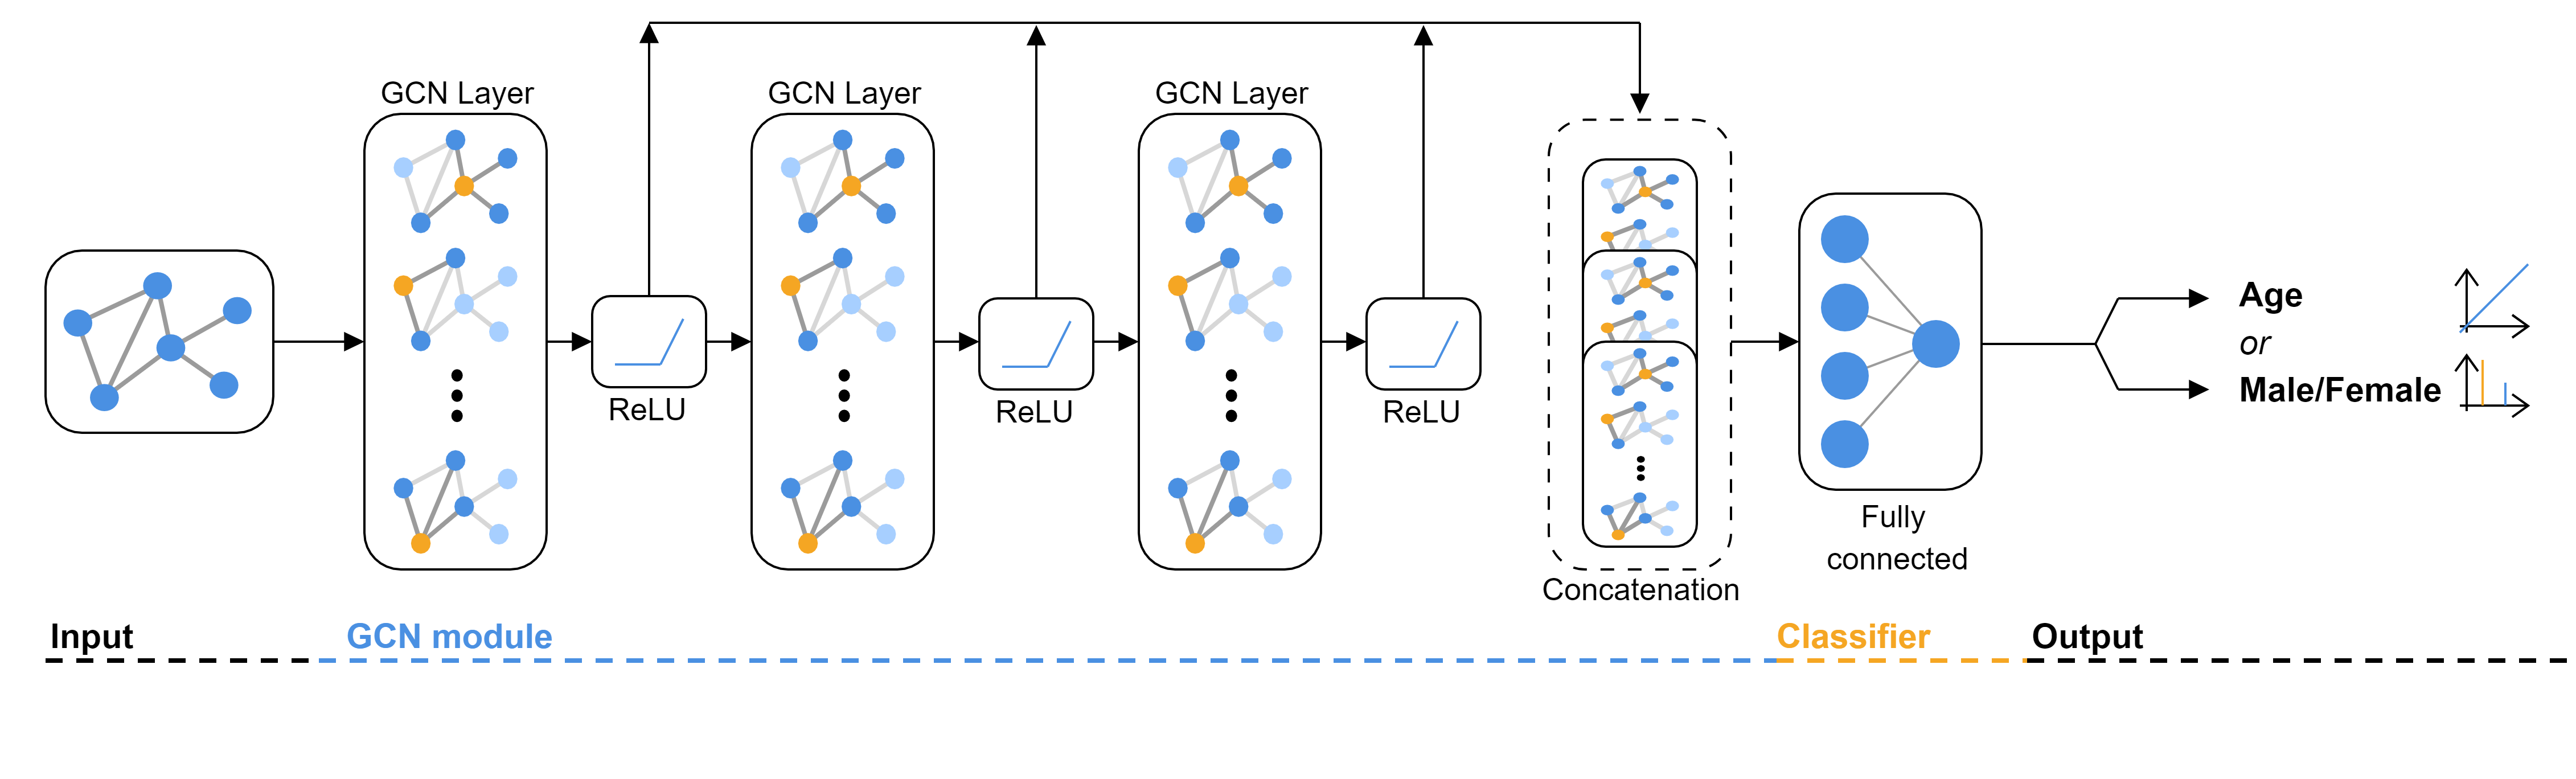
\includegraphics[width=\textwidth]{chapters/images_methods/base_v2.png}
    \caption{The GCN model, which takes a single brain graph as input and outputs a predicted age or sex. The input graph is processed through three graph convolutional layers with ReLU activation, afterwhich the activations after each layer is concatenated together and fed into a fully connected layer.}
    \label{fig:gcn_base}
\end{figure}


\section{Node classification -- population graphs}
In the next part of the thesis we investigate how well models involving population graphs perform. In this case since each node in the population graph is a subject the models need to do node predictions instead of graph predictions. 

\subsection{Forming population graphs}

As discussed in section \ref{sec:similarity_measure}, the design of the similarity measure is an important decision and should be done with the given application in mind. For our specific application, it's desirable that subjects that have similar fMRI data are connected with edges that have large weights, with the idea that the models will be able to draw upon this information of similarity to yield a better inference. A general construction that fulfils this requirement is the use of a distance metric inverted by a kernel as described in equation \eqref{eq:similarity_measure}. Following this approach, and given two subjects and their adjacency matrices $A_1$ and $A_2$, we define the similarity measure $\sigma\left(A_1, A_2, l\right)$ as
\begin{equation}
    \sigma\left(A_1, A_2, l\right) = \exp{\left(- \frac{||A_1 - A_2||_F^2}{l||A_1||_F ||A_2||_F} \right)}\biggr\rvert_{l=0.5},
    \label{eq:modified_similarity_measure}
\end{equation}
where $||A_1 - A_2 ||_F$ is the matrix Frobenius norm of the difference between $A_1$ and $A_2$. The Frobenius norm is defined as $||A||_F = \left( \sum_i \sum_j |A_{ij}|^2 \right)^{1/2}$. The norm of the difference is weighted with a hyperparameter $l=0.5$ and the norms of $A_1$ and $A_2$, and then fed into a Gaussian kernel. The Gaussian kernel ensures that larger differences between $A_1$ and $A_2$ yields smaller similarity scores $\sigma\left(A_1, A_2, l\right)$, and also that  $\sigma\left(A_1, A_2, l\right) \in \left[0, 1\right]$. As desired, subjects that have similar fMRI data, and thus a smaller difference between their adjacency matrices, will with equation \eqref{eq:modified_similarity_measure} obtain a larger similarity score and vice versa. 

Note that the similarity measure in equation \eqref{eq:modified_similarity_measure} only draws use of the fMRI data for each subject. One could imagine a similarity measure that uses other types of data that is related to the tasks of predicting age/sex, such as eventual brain-health related diagnosis \cite{stankeviciute}. The choice of only using fMRI data was motivated by two reasons; partly because using other data sources requires extensive domain knowledge, and partly because we are specifically interested in the predictive power of fMRI data, without introducing other confounding variables.

\subsection{Poptoy model}
As a first model for doing predictions on a population graph the Poptoy model is introduced. Poptoy takes in a population graph and propagates it through five graph convolutional layers, similar to GCN, but the output layer differs since Poptoy shall do node prediction instead of graph predictions. The output layer of Poptoy is still a fully connected layer with one or two softmax output neurons, but the input to the fully connected layer consists of the activations of all layers and all features for a specific node. This in contrast to GCN's output layer which takes the activations for all layers and all features for all nodes as input. By then using the same fully connected output layer for each node repeatedly (same weights) a prediction for each node, and thus each subject, can be made and the number of weights kept low as the number of nodes grows. An illustration of the Poptoy model can be seen in figure \ref{fig:poptoy}.

The reason the Poptoy model consisted of five graph convolutional layers instead of three, which GCN had, was that the population graphs became much larger then the individual brain graphs. The individual brain graphs consisted of 21 nodes which where all more or less connected and since each graph convolutional layer takes into account one higher order of neighbours the need for more graph convolutional layers quickly diminishes, since all nodes to some extent are included in the first order neighbourhood. For population graphs the need for considering neighbours further away in the graph might thus be much larger and hence Poptoy utilizes more graph convolutional layers then GCN. 

\begin{figure}[H]
    \centering
    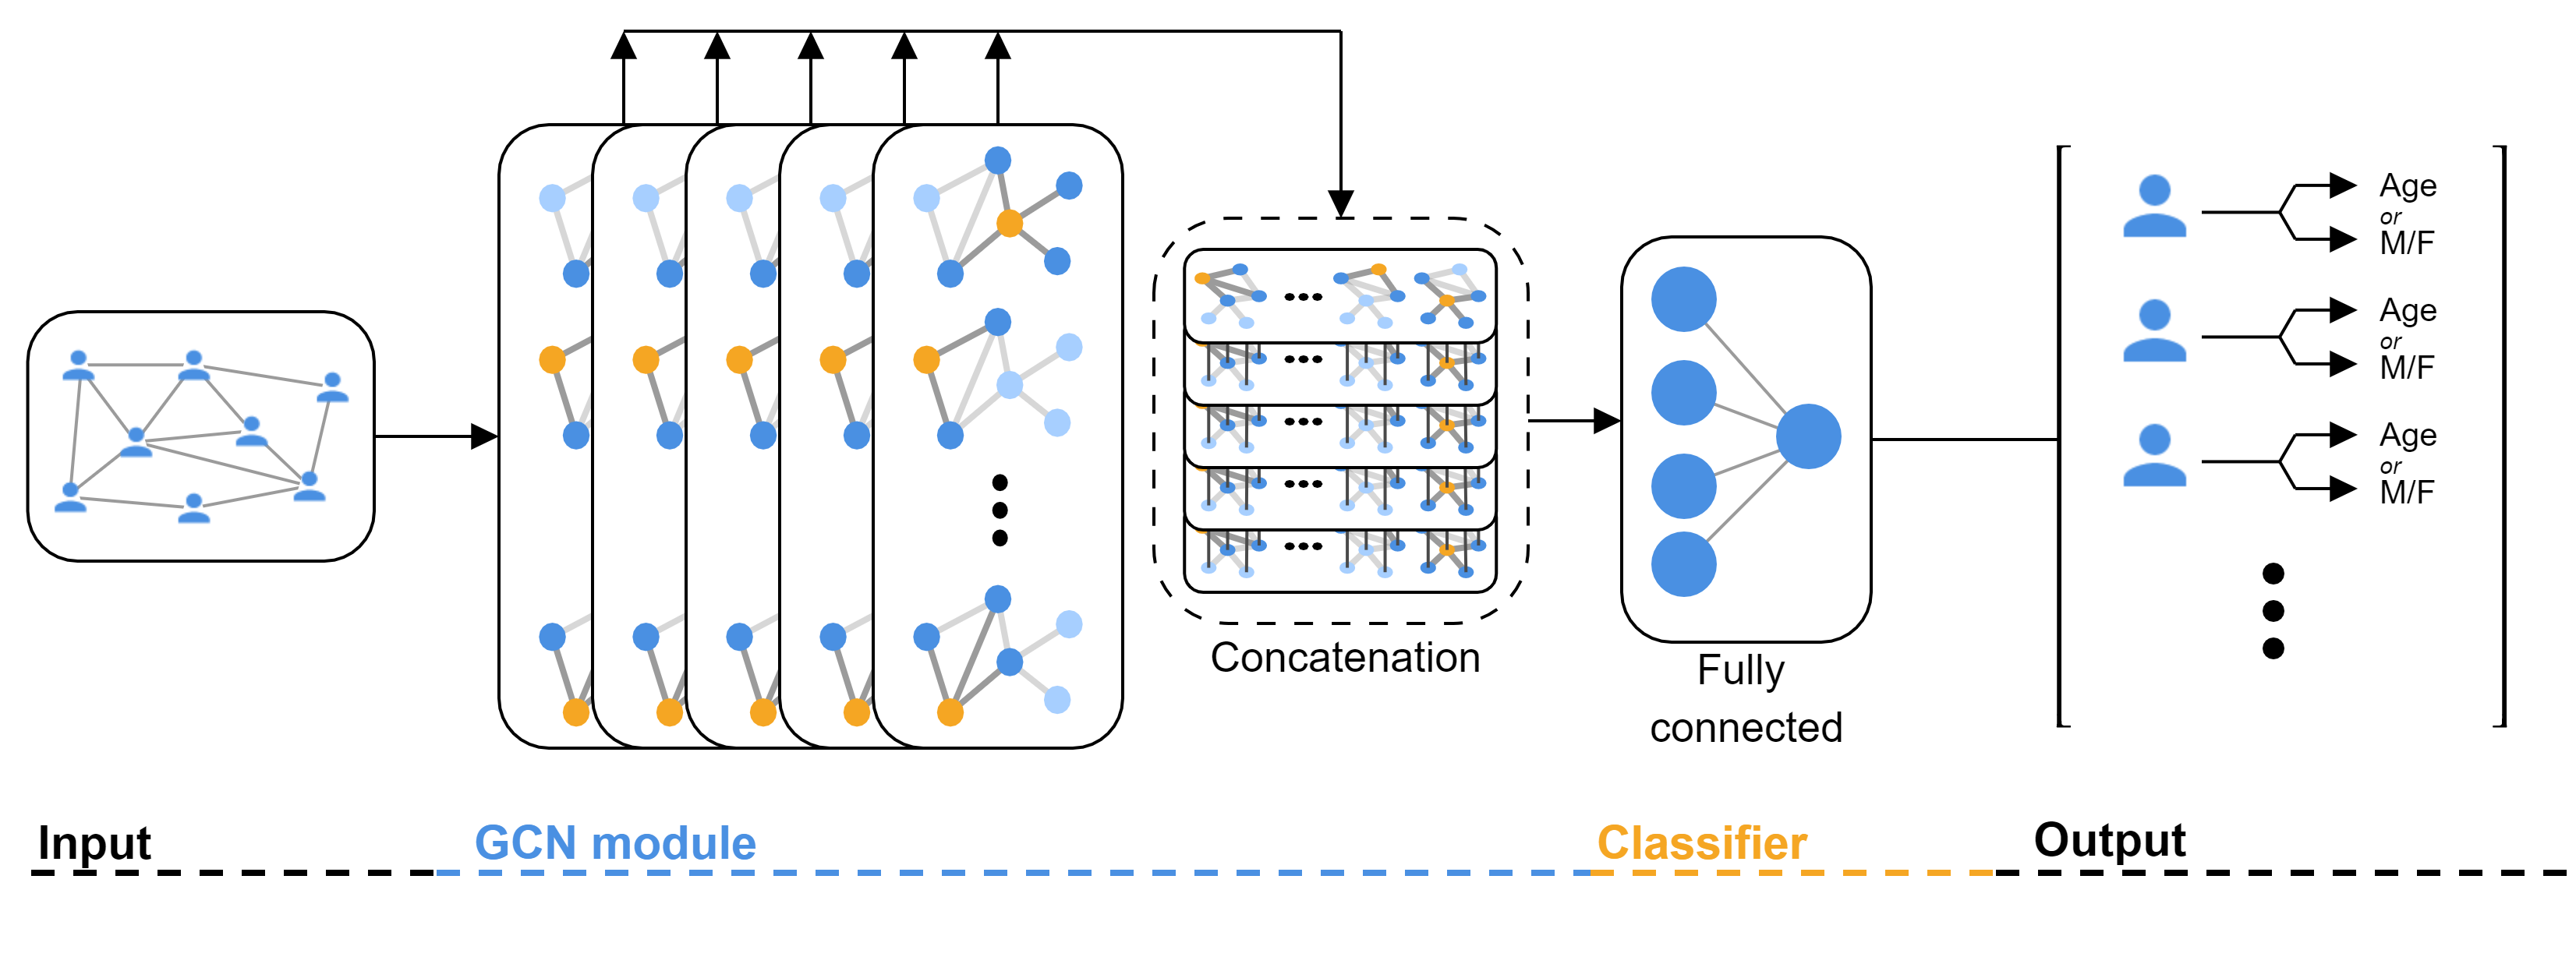
\includegraphics[width=\textwidth]{chapters/images_methods/poptoy_v2.png}
    \caption{The PopToy model. The input consists of a population graph, which is passed through five graph convolutional layers. The five activations are concatenated together and fed into a fully connected output layer, which outputs a predicted age or sex on a subject-level.}
    \label{fig:poptoy}
\end{figure}

Since all subjects in the data set are incorporated in the population graphs the split into validation and training set must be handled. The solution is given by defining a set of subjects that will be the training set and another that will be the validation set, and the population graph thus has one set of nodes considered to be training nodes and one set of validation nodes. The model was then constructed so it could either do predictions for only the nodes in the training set or validation set. Then the training could be performed while only doing predictions on the training set and vice versa when evaluating.

%\subsection{POPToy w. dummy}
%\subsection{POPToy w. features (fmri)}
\subsection{POPEncoder}
As a means to incorporate more information about each subject in the population graph a model referred to as POPEncoder was designed. The Popencoder model is identical to Poptoy in the sense that it propagates the population graph through five GCN layers and then makes a prediction for each node with a fully connected layer. The difference is that in Popencoder features for each node are introduced. The features are based on the adjacency matrices of each individual subject, but to compress the dimensionallity of the feature space these matrices was encoded into a lower dimensional space. The encoder consisted of two GCN layers with ten features each followed by a fully connected layers with two output neurons with a linear activation function. For an illustrations see figure \ref{fig:popencoder}.

A heuristic explanation of why the features introduced to the population graph would help, is that the encoder can make an initial prediction of the age or sex of each individual subject. Then by propagating this information through the population graph the information of similarities to other subjects in the data set possibly can improve on the predictions. One could argue that in that case the case that the initial prediction might be done as a preprocessing step, for example via a prediction with another model. The encoding is however viewed as a trainable part of the model and has has two output features to allow for more abstract and advantageous embeddings. 



\begin{figure}[H]
    \centering
    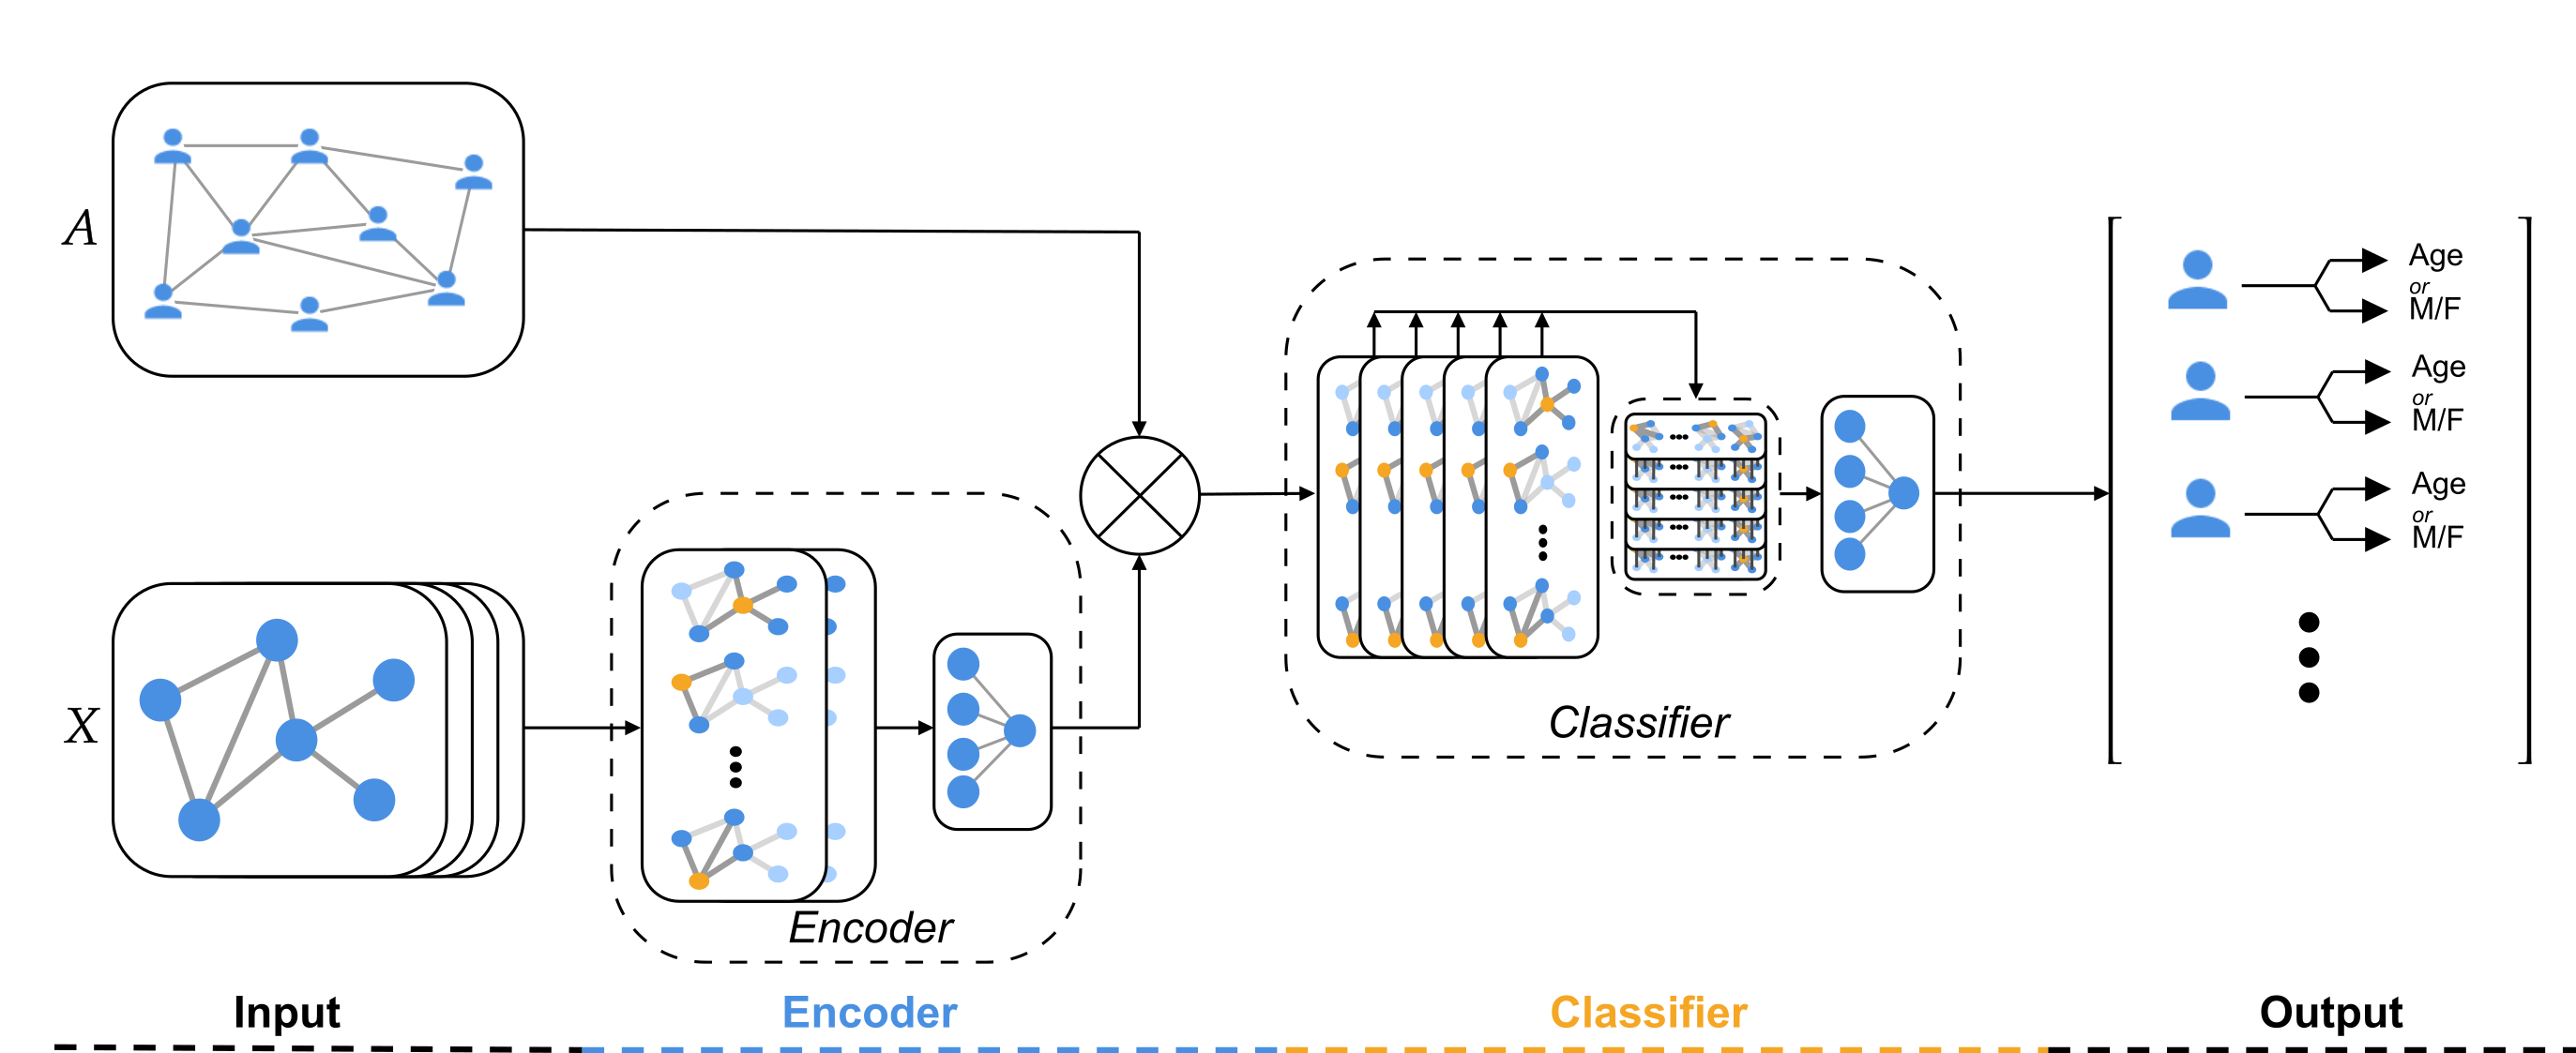
\includegraphics[width=0.9\textwidth]{chapters/images_methods/popencoder_v2.png}
    \caption{The PopEncoder model, which takes two inputs: a population graph $A$, and the brain graphs for all subjects in the population graph, $X$. The brain graphs are passed through an Encoder, consisting of two graph convolutional layers followed by a fully connected layer. The encoded brain graphs and the population graph $A$ are then fed into the Classifier, which consists of five graph convolutional layers followed by a concatenation and fully connected layer. The output is a predicted age or sex on a subject-level.}
    \label{fig:popencoder}
\end{figure}

\section{Batches of population graphs}
Since a population graph is a graph where each node represent a single subject and the number of edges of the graph grows with the number of nodes squared the adjacency matrix for the population graph quickly becomes very large. For example, a population graph with 30 000 nodes requires approximately 7 GB of memory to store. This is a problem since doing prediction and training with such a large matrix becomes time consuming and the memory consumption can also become problematic. To resolve this problem and thus in a feasible way be able to train models on population graphs that includes all the data a batching method was developed. 

\begin{figure}[H]
    \centering
    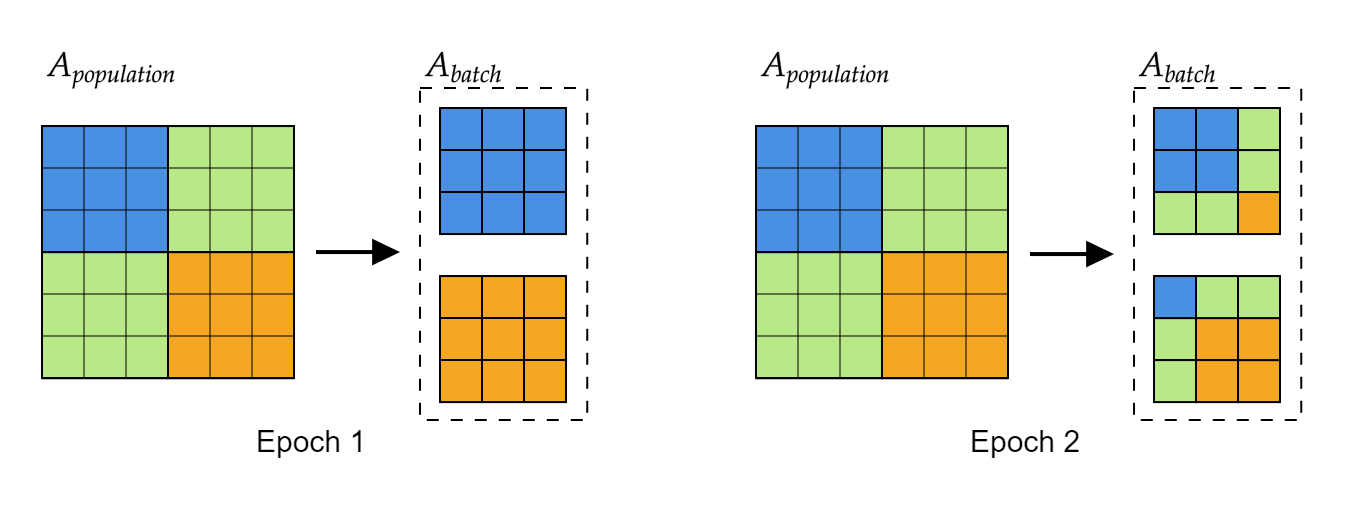
\includegraphics[width=0.9\textwidth]{chapters/images_methods/batches.png}
    \caption{An example of the batching approach for splitting a large population graph $A_{population}$ into two smaller population graphs, each corresponding to a batch $A_{batch}$. In Epoch 1, only the connections between the first three (blue) and last three (orange) subjects are included in the batched population graphs. By permuting which subjects are included in each of the smaller population graphs for Epoch 2 and onwards, all connections not included in the first epoch (gray) will eventually be sampled.}
    \label{fig:batches}
\end{figure}

The batching method was based on dividing the population graph into several smaller population graphs. This was done by splitting the data set into several smaller data sets of 100 subjects each and constructing one population graph for each data set. Practically this was done by extracting all connections between the 100 subjects from the larger population graph. For an illustration on how this was done see figure \ref{fig:batches}. With this batching approach, dividing a population graph of 30 000 subjects into 300 smaller graphs with 100 nodes each would require 24 MB of memory, as compared to 7 GB before batching. This is a difference of roughly two orders of magnitude.

As seen in figure \ref{fig:batches} many of the connection between subjects are not utilized if the population graph is divided into several smaller graphs. To solve this the way the subjects are divided into smaller graphs is changed between epochs as seen in figure \ref{fig:batches}. By always changing which people are combined in the graphs all connections will eventually be used after enough epochs. The advantage of always changing the subjects that are included in the graphs is that the model can't overfit against a specific graph structure. The models are thus forced to learn very general patterns to make predictions for all subjects in the graphs. However, this generalization might also become a disadvantage since overfitting on the graph structure may yield higher validation performance as long as the graph structure remains fixed. 


\section{Node importance analysis}
Since the goal of the thesis is not only to construct models to achieve good performance, but also to determine what functional networks in the brain are related to sex and age, analysing the models is an essential part of the work. Specifically, analysing which nodes in the brain graph are important for making predictions will by extension give information on what functional networks are important, due to each node representing a functional network. 

Two black box methods for model analysis will be used: a naive approach based on node removal, and a more sophisticated method for node masking based on the Zorro algorithm described in section \ref{sec:zorro}. Black box methods are beneficial in this case, since they pose no assumptions on the model architecture, only on in- and output, and thus the analysis may be performed for different models in order to validate and compare the results. 

\subsection{Naive approach - Impact of node removal on performance}
A simple method to investigate which nodes are important for doing predictions is a node removal method. This particular method is self-composed, and based on simply removing a specific node for every subject in the data set and then retraining a new model. By comparing the predictive performance of the retrained model with a reference model trained on data with all nodes intact, an indication of the importance of that node may be obtained. This is the case since a large loss in performance means vital information for the prediction was removed, which is interpreted to be indicative of the importance of that node. The method may then be repeated for all nodes in order to obtain a measure of how important each node is.

\subsection{Zorro}

The Zorro algorithm which is described in \ref{sec:zorro}, was developed for semi-supervised learning on a node classification task. To be used for analysing the models considered in this thesis it thus needs to be modified.

The need for modification arises since the Baseline and Base models are completely featureless approaches that only takes an adjacency matrix as input. Therefore it is not possible to mask the feature matrix and it must be done on the adjacency matrix. The unmasking can be done in two ways; either on a connection level where entries in the adjacency matrix are unmasked or on a nodal level were whole rows and columns in the matrix are unmasked. Since we primarily where interested in which nodes are important the latter was used. Masking whole nodes instead of connections also give computational benefits, since the number of nodes is much less then the number of connections. 

An explanation $\mathcal{S} = \{V\}$, thus now only contains a set of nodes to be unmasked. The masked adjacency matrix is now given by 
\begin{equation*}
    B_S = A \odot S + Z \odot (1- S), \quad Z \sim \mathcal{N},
\end{equation*}
where $S$ is the masking matrix for the explanation $\mathcal{S}$, and the model predictions are $\Phi(A)$ and $\Phi(B_S)$. For age prediction, $\Phi(B_S)$ was deemed correct if $\left|\Phi(A) - \Phi(B_S)\right| < t$ for some tolerance $t$, since age is a continuous variable. In our implementation, $t$ was set roughly correspond to the MAE of the models. The noise is drawn from a Gaussian distribution with mean and standard deviation given by the entries of $A$ over the data set. The fidelity is calculated in the same way as in the original algorithm, and an explanation $\mathcal{S}$ for an individual subject is still accepted if the fidelity of $\mathcal{S}$ is higher then $\tau$. 

Lastly, since the algorithm yields which nodes are important for the prediction of an individual subject, the procedure was repeated for several subjects to get a sense of which nodes are generally important. To evaluate the importance of each node an importance score $\mathcal{I}$ was introduced as the number of explanations $\mathcal{S}$ a node was included in, divided by the total number of subjects. An importance score of $\mathcal{I}=1$ indicates that the node was considered important for the prediction of all subjects, and a score of $\mathcal{I}=0$ for none.  


% \subsection{Salience mapping, GRAD-CAM}
% Another method not utilizing different kinds of masking algorithms is the GRAD-CAM method which is a method for opening up the black box. The basic principle of the GRAD-CAM algorithm is to study activations of different graph-nodes in the model when predictions are made. By identifying the nodes where the activations impact the predictions the most important graphs-nodes can be identified. 

% The GRAD-CAM algorithm was initially made for convolutional neural network where important pixels in an image was identified \cite{} but was generalized to GCNs in \cite{}. The algorithm calculates the importance score for node $n$ at the GCN layer $l$, for class $c$ by 
% \begin{equation*}
%     L_c[l,n] =  \text{RELU}(\sum_k \alpha^{l, c}_k F_{K,n}^l). 
% \end{equation*}
% Here $F_{K,n}^l$ is the activations of the $k$-th feature of the $l$-th GCN layer at node $n$ and $\alpha^{l, c}_k$ is a set of class specific weights for layers $l$ given by 
% \begin{equation*}
%     \alpha^{l, c}_k = \frac{1}{N}\sum_{i = 1}^N \frac{\partial y^c}{\partial F^l_{k,n}}.
% \end{equation*}

% This algorithm depends on the architecture of the model having a GAP layer between the last GCN layer and the fully connected output layer. A GAP layers is average global pooling layer which averages all the features of the last layer over the nodes before passing them to the dens layer. This is a big problem since GCNBase has primarily two significant differences. The first one being that GCNBase does not utilize any GAP layer before the output layer and thus has a specific weight for all nodes and features not only one weight per feature. The second problem is that GCNBase in addition to the activations of the last GCN layer also utilizes the activations of all previous GCN-layers. The solution to these problem is to do some slight alterations to the GRAD-CAM algorithm in the form of 
% \begin{equation*}
%     L_c[l,n] =  \text{RELU}(\sum_k \alpha^{l, c}_{k,n} F_{K,n}^l)
% \end{equation*}
% and
% \begin{equation*}
%     \alpha^{l, c}_k = \frac{\partial y^c}{\partial F^l_{k,n}}.
% \end{equation*}
